% options:
% thesis=B bachelor's thesis
% thesis=M master's thesis
% czech thesis in Czech language
% slovak thesis in Slovak language
% english thesis in English language
% hidelinks remove colour boxes around hyperlinks

\documentclass[thesis=B,english,hidelinks]{FITthesisXE}[2012/06/26]
\usepackage[utf8]{inputenc} % LaTeX source encoded as UTF-8
\usepackage{xeCJK}
\setCJKmainfont{Yasashi.ttf}

\usepackage{graphicx} %graphics files inclusion
\graphicspath{{images/}}
% \usepackage{amsmath} %advanced maths
% \usepackage{amssymb} %additional math symbols

\usepackage{dirtree} %directory tree visualisation
\usepackage{listings}

\lstset{ %
  backgroundcolor=\color{white},
  basicstyle=\footnotesize,
  breakatwhitespace=false,
  breaklines=true,
  captionpos=b,
  deletekeywords={...},
  escapeinside={\%*}{*)},
  extendedchars=true,
  rulecolor=\color{black},
  showspaces=false,
  showstringspaces=false,
  showtabs=false,
  tabsize=2
}

% % list of acronyms
% \usepackage[acronym,nonumberlist,toc,numberedsection=autolabel]{glossaries}
% \iflanguage{czech}{\renewcommand*{\acronymname}{Seznam pou{\v z}it{\' y}ch zkratek}}{}
% \makeglossaries

\newcommand{\tg}{\mathop{\mathrm{tg}}} %cesky tangens
\newcommand{\cotg}{\mathop{\mathrm{cotg}}} %cesky cotangens

\department{Department of Software Engineering}
\title{Educational turn-based RPG}
\authorGN{Tomáš} %(křestní) jméno (jména) autora
\authorFN{Havlík} %příjmení autora
\authorWithDegrees{Tomáš Havlík} %jméno autora včetně současných akademických titulů
\supervisor{Ing. Miroslav Balík, Ph.D.}
\acknowledgements{I would like to extend my thanks to my supervisor, Ing. Miroslav Balík, Ph.D., for his support in leading this thesis, my good friend and Kanji Adventure co-creator David Nguyen for his part in bringing the virtual environments to life, my parents Věroslav and Lenka for supporting me during my studies and Jakub Jirůtka for letting me use a modified version of his \XeLaTeX ~class file. I would also like to thank Marián Hlaváč, Anna Zderadičková and Veronika Judáková for helping out during the testing phase. Last but not least, I would like to thank the awesome developers at Defold for providing fast and concrete answers to many development-related questions.}
\abstractCS{Cílem bakalářské práce je vytvoření funkčního prototypu tahové hry na hrdiny s výukovými prvky. Popisuje použité konvenční herní a výukové postupy a snaží se vytvořit unikátní kombinaci mezi tahovým bojovým systémem a dynamickým výukovým systémem, který zkouší uživatele ze čtení japonských znaků. Znaky se vybírají na základě chybovosti.}
\abstractEN{The aim of this bachelor thesis is to create a functional prototype of an educational role-playing game. It introduces conventional gameplay and educational practices used and attempts to create a unique synergy between the turn-based combat system and a dynamic learning system, which queries the user on readings of Japanese characters. The latter is tailored to the specific player --- characters are chosen depending on past mistakes.}
\placeForDeclarationOfAuthenticity{Prague}
\declarationOfAuthenticityOption{1} %volba Prohlášení (číslo 1-6)
\keywordsCS{rpg, videohra, výuková, analýza, návrh, implementace}
\keywordsEN{rpg, videogame, educational, analysis, design, implementation}

\bibliography{bibliography.bib}

\begin{document}

% \newacronym{CVUT}{{\v C}VUT}{{\v C}esk{\' e} vysok{\' e} u{\v c}en{\' i} technick{\' e} v Praze}
% \newacronym{FIT}{FIT}{Fakulta informa{\v c}n{\' i}ch technologi{\' i}}

\begin{introduction}

\tolerance=1
\emergencystretch=\maxdimen
\hyphenpenalty=10000
\hbadness=10000

Modern technologies enable students to acquire new language skills with relative ease compared to traditional means. Many have taken up this opportunity and released pioneering educational software, which takes advantage of contemporary personal computers and, perhaps most importantly, smart devices. Although a lot of these products employ features that make them appealing to use, few come close to immersion found in~traditional videogame products, a characteristic which is of paramount importance to user retention and in turn effectiveness of these solutions in~the~long term.

The purpose of this thesis is to draw from the best game design, programming and educational practices and to ultimately create a prototype of a full-fledged interactive videogame experience that facilitates learning Japanese kanji~characters.

The game is a joint project between myself and my friend David Nguyen\autocite{nguyen}, a student of Art \& Design at Prague College, who is involved in the process of~creating the vast majority of graphical assets used within the game.

\section{Japanese writing system}

In this subsection we introduce the Japanese writing system. Contemporary Japanese language makes use of the following three types of scripts in addition to Latin characters.

\subsection{Kanji}

Kanji are adopted logographic Chinese characters. They are the main building blocks of Japanese language used to refer to most objects and actions. In~contrast with Chinese, which features only one way of pronunciation, Japanese includes two distinct styles of reading --- \emph{on'yomi} and \emph{kun'yomi}\autocite{literacy}. The on'yomi reading refers to a phonetic approximation of the original Chinese pronunciation, whereas kun'yomi is the Japanese reading of kanji. Kun'yomi are generally used when the kanji is present either in a stand-alone manner or in combination with hiragana characters. This use case can be observed~in~most verbs. On'yomi, on the other hand, are used in kanji compounds.

\subsection{Hiragana}

Hiragana is one of the two syllabaries used in Japanese\autocite{literacy}. It is used in forming grammatic constructs and additionally can be utilised in place of kanji for~obsolete or more difficult kanji in the form of \emph{furigana}. This practice is common with academic textbooks for younger students and non-native speakers.

\subsection{Katakana}

Katakana is the other Japanese syllabary\footnote{A set of written characters each of which is used to represent a syllable\autocite{merriamsyllabary}.} used exclusively for transcription of~words originated in other languages, most commonly English and German\autocite{literacy}. Some words are not transcribed into katakana, but are instead written using their original Latin form.

\newpage

\section{Chapters}

The thesis is comprised of the following chapters.

\subsection{Analysis}

In this chapter we analyse examples of gaming and non-gaming software products that aim to teach the user Japanese in one form or another. We~discuss their learning elements and game mechanics or \emph{gamification}\footnote{Gamification is the process of applying game design practices into non-gaming applications.} elements that support the educational framework. We also take a look at two examples from the turn-based role-playing game genre and analyse their combat mechanics. We conclude the chapter by selecting features that would form the~basis~for~our~game.

\subsection{Requirements}

Includes specification of functional and non-functional requirements for~our~game.

\subsection{Technology}

In this chapter we introduce tools that are used during development of~the~game. We take a look at the game engine used and some of the reasons behind choosing it, the external map editor and the reasoning as to why use one, data storage formats for storing many structures included within the~game and a~version control system used during development.

\subsection{Battle system}

Includes description of combat mechanics, the learning and the challenge systems used in the game, a diagram detailing communication between components and a detailed description of these components and data structures exclusive to the battle portion of the game.

\subsection{Exploration system}

Details the questing system used within our game, introduces the item system and item economy and talks about the experience system. As with the~battle chapter, we discuss data structures and script components exclusive to~this~part~of~the~game.

\subsection{Shared elements}

Contains information on data structures and script components used outside of~and~in~both the battle and exploration parts of the game. Details~the~persistence module and the used tile rendering algorithm.

\subsection{Tutorial}

Details the process of introducing the player to key gameplay mechanics via~a~series of images that guide the player to perform specific actions.

\subsection{Testing}

Includes lessons learned from user testing the game on three individuals.

\subsection{Future additions}

This chapter details some of many possible ways of improving the game.

\end{introduction}

\chapter{Existing products}

\tolerance=1
\emergencystretch=\maxdimen
\hyphenpenalty=10000
\hbadness=10000

In this chapter we will introduce some of the many examples of non-gaming educational applications as well as a couple educational videogames that we draw expertise from when designing the educational element of our videogame. Also mentioned are examples of the role-playing game genre that include turn-based combat. We conclude the chapter by selecting features that would form the basis for our game.

\section{Non-gaming applications}

There is currently an abundance of non-gaming applications available on~the~market that utilize spaced repetition for learning purposes. The most popular examples are \emph{Anki}\autocite{anki}, \emph{Memrise}\autocite{memrise}, \emph{Duolingo}\autocite{duolingo} and \emph{Wanikani}\autocite{wanikani}, just to name a few. Apart from Anki, which is a lightweight application with a do-it-yourself approach, all of these applications include a gamification element, which gratifies the learner by providing virtual badges, leaderboards and progress indicators. These functions are geared towards stimulating competitiveness, a basic human trait, which in turn keeps the player coming back for more.

\subsection{Memrise}

\subsubsection{Learning element}

Content in Memrise is divided into languages, which are further divided into~courses made and maintained by end users. Learner can associate a~course with their account and be notified each day when it is time to practice. This~mechanism helps maintain knowledge. Users interact with the learning system in the following ways:

\begin{itemize}
\item learning mode --- the session consists of repeated queries on a number of~new~phrases,
\item review mode --- player is given a set of queries on phrases that have not been practiced lately,
\item speed review --- introduces stricter time constraints,
\item my difficult words --- the session consists of queries on phrases that the~player struggles with.
\end{itemize}

As we can see, the system includes two primary modes of repetition --- one that selects phrases depending on time passed since last review and one that selects phrases that have been entered incorrectly a large amount of times.

\begin{figure}[ht]
\centering
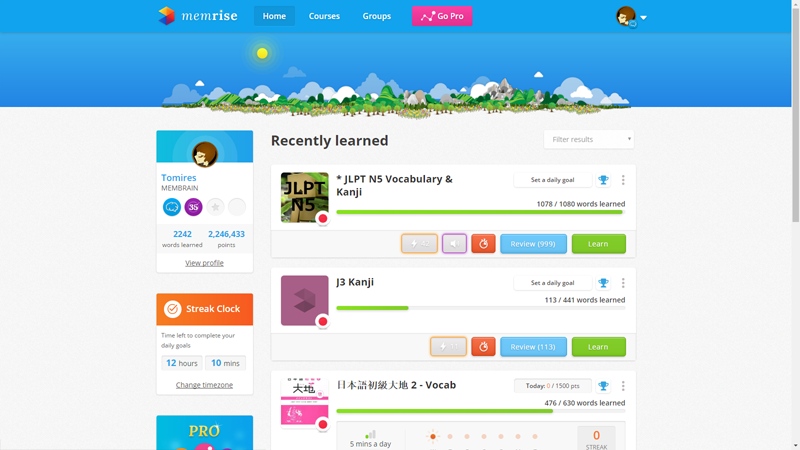
\includegraphics[scale=0.45]{memrise}
\caption{Memrise user interface}
\label{fig:memrise}
\end{figure}

\subsubsection{Gamification}

Memrise places emphasis on community features. The user can browse through profiles of other individuals, check on courses they have started, view custom-made educational memes\footnote{Meme is an idea, behavior, style, or usage that spreads from person to person within a culture.\autocite{merriammeme}} that they have created and see a tally of~words they have learned and points they have amassed.

Points are also prominently visible in leaderboards, which are displayed on~course pages. The aforementioned features introduce competitiveness between players.

Another gamification feature used is called ``Streak Clock'', which grants the~player additional points and badges for their profile for learning a specified amount of new words every day. This motivates the player to play regularly, which is of upmost importance in educational applications of this type.

\subsection{Duolingo}

\subsubsection{Learning element}

In contrast with Memrise, Duolingo offers a unified learning experience for~each language. Courses place a significant emphasis on grammar and are divided into sections, which are further divided into lessons. Progress through sections is strictly linear. In order to unlock the next section, the user has to~first complete a set number of lessons and pass a revision test.

In addition to the learning experience, there is also a review mode, which works the same as in Memrise's case.

\begin{figure}[ht]
\centering
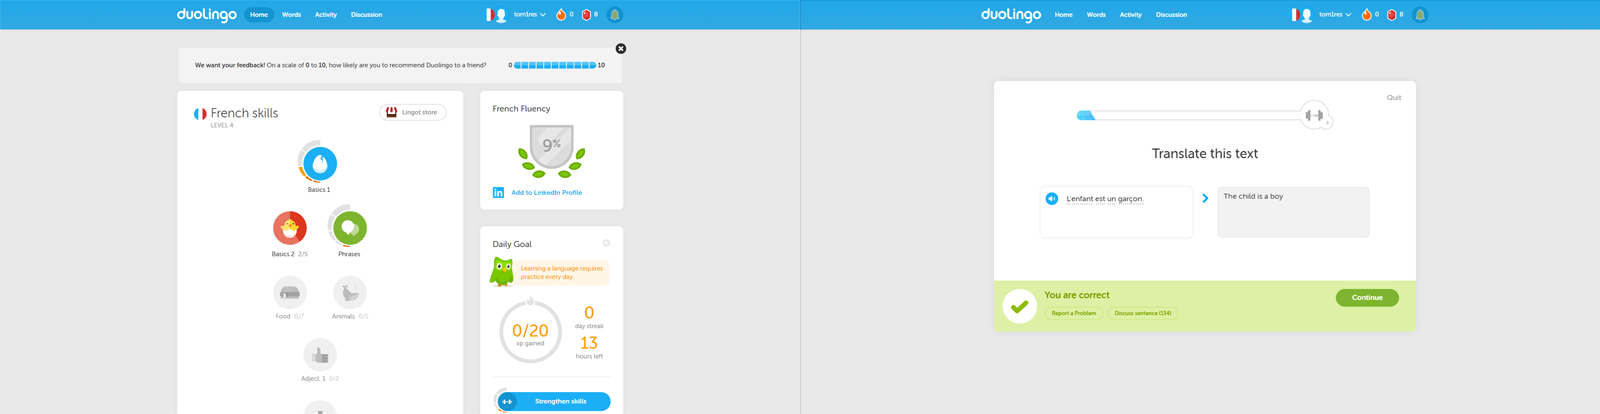
\includegraphics[scale=0.45]{duolingo}
\caption{Duolingo user interface}
\label{fig:duolingo}
\end{figure}

\newpage

\subsubsection{Gamification}

Duolingo includes most, if not all, gamification elements of Memrise. A~``Daily~Goal''~system is present and rewards users with ``lingots'', a form of~virtual currency that unlocks additional challenges. Community features are for~most~part limited to user's friends, the system includes an activity feed that highlights user progression and is viewable by others.

\subsection{Wanikani}

\subsubsection{Learning element}

The user interface of Wanikani is rather different from the previous two examples. The learning experience consists of learning radicals (building blocks of kanji characters), utilising said radicals in kanji and ultimately combining kanji characters into vocabulary. Although the idea of building blocks appears solid, the application feels more like an encyclopaedia rather than a learning program and the testing functions look spartan compared to~the~aforementioned examples and feel like an afterthought.

\begin{figure}[ht]
\centering
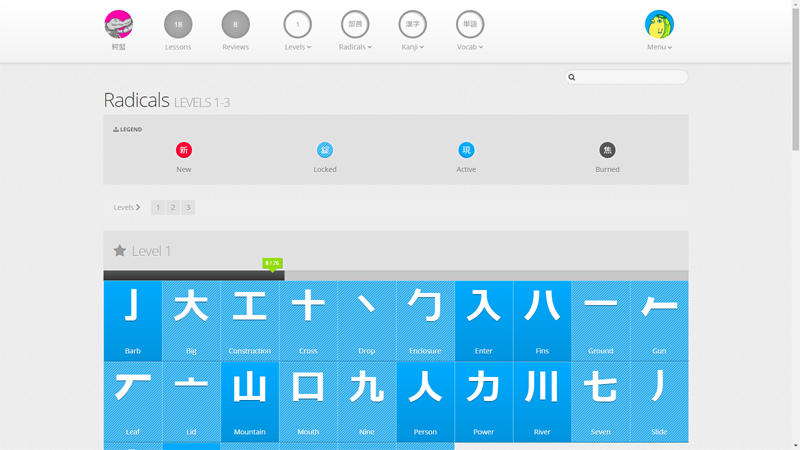
\includegraphics[scale=0.45]{wanikani}
\caption{Wanikani user interface}
\label{fig:wanikani}
\end{figure}

\subsubsection{Gamification}

As with Memrise and Duolingo, Wanikani includes a profile system, which shows user's progression through various stages (Apprentice, Guru, Master and so on) and includes few other basic statistics. Compared to other learning systems, Wanikani's gamification elements are very basic.

\section{Gaming applications}

The realm of gaming applications that are focused on teaching Japanese is~comparatively small. It is very important to distinguish between true gaming experiences and simple mechanics borrowed from the gaming industry. For~example, there is a number of ``games'', whose sole gaming mechanic is~the~concept of hit points with no further interactivity other than selecting answers to queries. For the purpose of this thesis, we will not classify these applications as games, but rather as non-gaming applications with a~gamification element. We have selected three examples that can be thought~of~as~videogames~in~their~own rights\autocite{fude}\autocite{owari}\autocite{hirbattle}.

\subsection{Fude Samurai}

\subsubsection{Learning element}

In order to execute special attacks, the player has to draw a kanji character with a correct stroke order. The player also encounters small mini games along the~way which include tasks such as putting kanji characters representing numbers in correct numerical order. The queries get progressively harder the~longer the~player practices the kanji in question. In the first phase, they are guided by outlines of the character, afterwards they have to make do with stroke order. In the final phase, the game gives them a blank slate. The training mode which can be accessed via the main menu allows the player to practice kanji independently from their progress in the story mode.

\begin{figure}[ht]
\centering
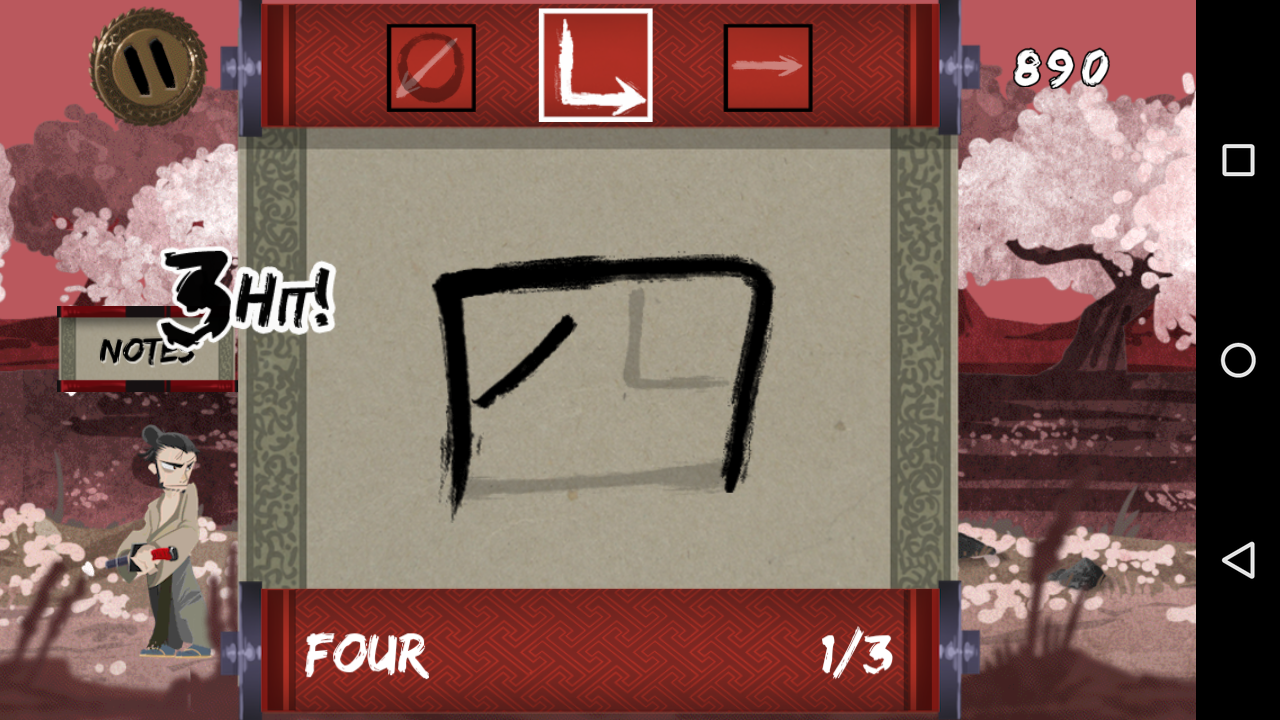
\includegraphics[scale=0.45]{fude1}
\caption{In-game screenshot from Fude Samurai}
\label{fig:fude}
\end{figure}

\subsubsection{Game mechanics}

Fude Samurai is a one button fighter designed with mobile controls in mind. The game is relatively simple to control and rewards fast reflexes rather~than~strategy.

\subsection{Kanji no Owari}

\subsubsection{Learning element}

At set intervals throughout the level, the player is presented with a review screen that highlights on'yomi and kun'yomi readings for a set number of kanji characters. These kanji characters then appear in queries that the player must answer in order to defeat incoming waves of enemies. It appears that every level includes a predetermined set of kanji for the player to practise.

\begin{figure}[ht]
\centering
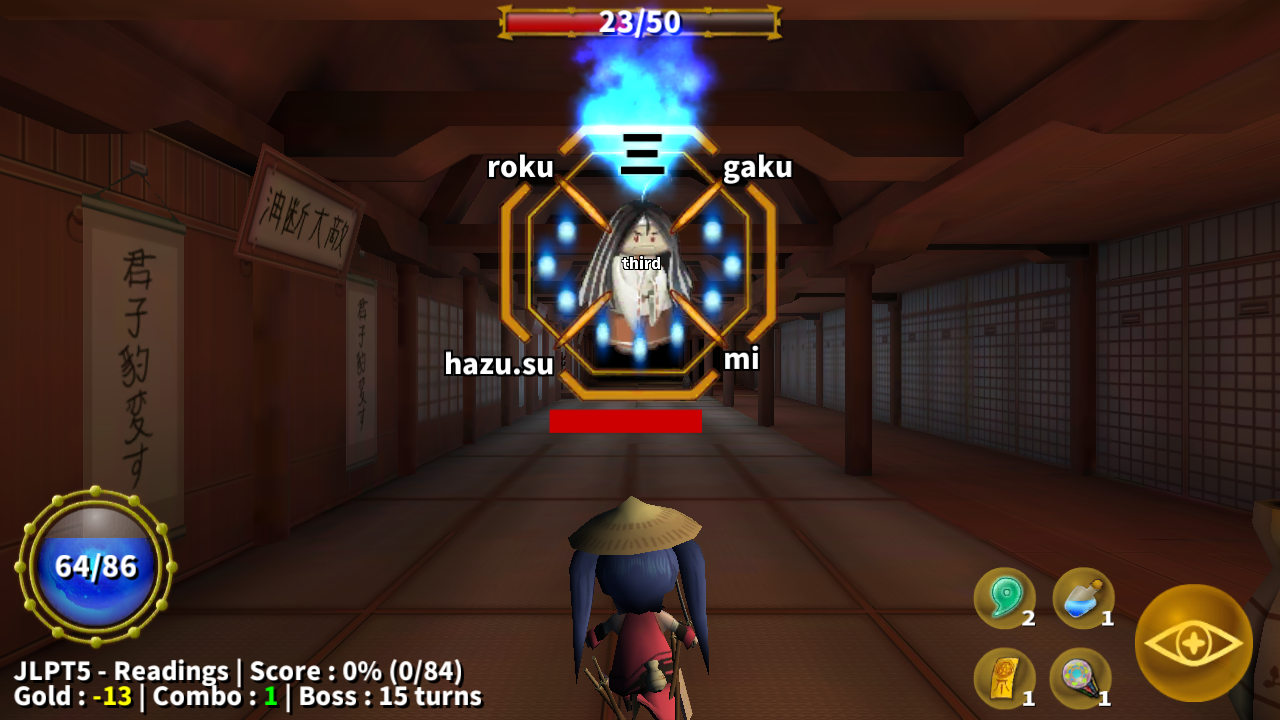
\includegraphics[scale=0.45]{owaru1}
\caption{In-game screenshot from Kanji no Owari}
\label{fig:owaru}
\end{figure}

\subsubsection{Game mechanics}

According to the developers, Kanji no Owari is a role-playing game. While it includes certain elements typical for RPG games, such as variable (and~upgradeable) statistics, the effect on gameplay is rather insignificant. Players amass virtual currency through play, which they can use to buy items that help them progress through levels, for example a vial that replenishes health. Gameplay revolves around defeating monsters by answering quickly to queries. At the end of each level, the player faces a boss enemy, which differs from other kinds of enemies by possessing a large amount of health points, therefore increasing the number of queries generated.

\subsection{Learn Japanese To Survive! Hiragana Battle}

\subsubsection{Learning element}

Unlike the rest of the games mentioned, the player is taught hiragana instead of kanji. Players are taught new syllables in sets of five during dialogues with~NPCs. They are also shown the pronunciation, draw order, albeit in a~non-interactive fashion. Immediately afterwards, they are tested on the newly gained knowledge via a series of queries. Hiragana characters appear in battles as enemies. The player is required to enter correct transcription in Latin script for each character to have a chance at inflicting damage using weapons or spells. The game also includes a quest system, which teaches the player a small amount of vocabulary and factual information about Japan.

\begin{figure}[ht]
\centering
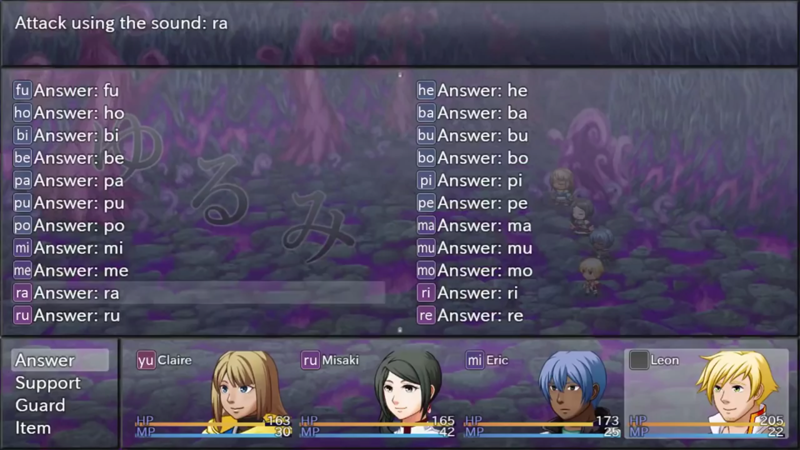
\includegraphics[scale=0.6]{hirbattle}
\caption{In-game screenshot from Learn Japanese to Survive! Hiragana Battle}
\label{fig:hirbattle}
\end{figure}

\subsubsection{Game mechanics}

The game is similar in play style to earlier entries in the Final Fantasy series. Players conduct turn-based battles in a traditional JRPG style. Battles take place at random intervals throughout the exploration experience, a mechanic often referred to in the gaming circles as a ``random encounter''.

\section{Turn-based role playing games}

The following two examples have been chosen to illustrate different approaches to a turn-based RPG, the variations of which are used in virtually every game in the genre. The first example allows for \emph{one action per turn} (per~character), while the second lets the player take \emph{multiple actions} over the~course of~a~turn\autocite{fireemblem}\autocite{dofus}.

\subsection{Fire Emblem}

The game features a battle system that alternates between the player and the~AI. Both sides possess control over multiple characters and as such can move and execute actions with each individual character. The routine is as follows --- player first moves the character to a new location and then has the option to either do nothing, attack using a weapon, use a spell or utilise an item. After performing an action, the character is deactivated for the rest of~the~turn. Attacks do not feature any kind of randomness, damage value is strictly determined by statistics of each character. These statistics are improved when the character levels up, the stat distribution is pre-determined to the best of our knowledge. When performing an offensive action, the target has a~chance to~execute a counter-attack. This depends on the character type. Melee characters cannot counter ranged attacks and characters that have received a~fatal blow aren't given a chance to fight back.

\begin{figure}[ht]
\centering
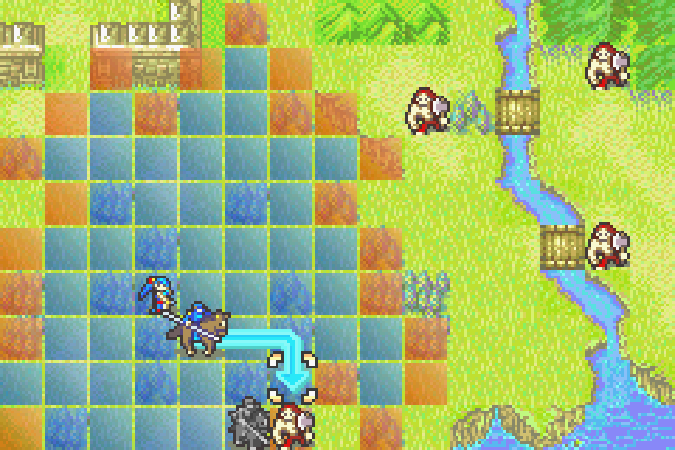
\includegraphics[scale=0.4]{fire1}
\caption{In-game screenshot from Fire Emblem}
\label{fig:fire}
\end{figure}

\subsection{Dofus}

This massively multiplayer online role-playing game contains a world populated by other players. As such, many elements of the battle system are designed to accommodate this fact. Turns have a time limit and there is an~entire category of spells used to help friendly characters. Each player has a~set amount of movement points and action points (APs) that they can utilise on~each turn. Individual spells have an AP cost and some have a cooldown, which prevents them from being used in subsequent turns. Each individual player controls only one character. Although some character classes are capable of summoning friendly characters, these are controlled automatically. The game includes an in-battle \emph{challenge system}, which rewards players for completing certain objectives, such as killing a certain enemy first or not losing any health throughout the fight.

\begin{figure}[ht]
\centering
\includegraphics[scale=0.45]{dofus}
\caption{In-game screenshot from Dofus}
\label{fig:dofus}
\end{figure}

\newpage

\section{Feature selection}

When it comes to picking phrases, we can either place focus on time since last revision or the number of mistakes in the last couple revisions. Due to the fact that answering queries forms an integral part of the game, we can ignore the~time vector as the player has to answer queries in order to progress in~the~game. If they stop, so does the game's progression.

One thing that we would like to borrow from Wanikani is the \emph{encyclopaedic feel}. The game should include an interface that lists kanji that the player has unlocked and phrases associated with said kanji.

All three non-gaming applications place great deal of attention to gamification elements which stimulate the player. We would like to introduce \emph{online profiles} in one of the expansions to the game.

When it comes to gaming applications mentioned, we cannot draw from their game design as they come from different videogame genres. We can however take note of mechanics they use to introduce new kanji to the player. Fude Samurai's story mode introduces new kanji gradually by guiding the player through stroke order. As the game places emphasis on teaching the player how to draw kanji characters, it does not need to explain pronunciation in~much~detail. If the player gets lost, they can practice in the training mode.

\newpage

Kanji no Owari seems to be lacking in the learning department. The whole experience seems to be geared towards players familiar with kanji who only need a quick revision. Hiragana Battle seems to include the best learning experience out of the three games mentioned. Thanks to the link with NPCs and story, the learning progression is gradual and does not feel forced.

Lastly, we need to choose between the two approaches to turn-based role-playing games. As we only control one character, the mechanics used in~Dofus seem to be a better fit for our game. The query mechanism needs to~be~linked to a frequently used gameplay mechanic. The most frequently used action in~Dofus seems to be spell casting. Thanks to the ability to cast multiple spells per turn, the frequency of queries is higher than it would be~if~we~opted~to use Fire Emblem's approach.

Two other mechanics in Dofus that we would like to use are the in-battle challenge system and idols, which are items used to modify battle conditions to~make them more challenging for seasoned players in exchange for~additional rewards. We would like to utilise this feature in our equipment system.

\chapter{Requirements}

\tolerance=1
\emergencystretch=\maxdimen
\hyphenpenalty=10000
\hbadness=10000

This chapter includes specification of functional and non-functional requirements for our game.

\section{Functional}

\subsection{Educational system}
The game needs to be able to effectively transfer knowledge of Japanese kanji onto the player.

\subsection{Battle system}
The battle system needs to facilitate frequent use of the educational element.

\subsection{Immersion}
The game needs to motivate the player in a way that does not involve improving their proficiency in Japanese, such as with well-paced quest arcs.

\subsection{Pick up and play}
Due to its semi-casual nature, the game needs to be able to support short gameplay sessions.

\subsection{Reward system}
The game should include an item system that gives the player a~sense~of~progression.

\section{Non-functional}

\subsection{Accessibility}
The game should be accessible to casual players and therefore abstain from using overly complex mechanics. It should communicate its mechanics in~a~clear visual form and provide a quick interactive tutorial for newcomers.

\subsection{Supportability}
Due to its aforementioned educational requirements, the game should be readily available to the player at any time. Targeted platforms include tablets and personal computers.

\chapter{Technology used}

\tolerance=1
\emergencystretch=\maxdimen
\hyphenpenalty=10000
\hbadness=10000

This chapter includes tools utilised during development of the game and discusses motivations behind choosing individual parts of the development stack.

\section{Defold}

Going into development, we had three basic requirements for the programming tool used in the process. First, it has to support all major desktop and mobile platforms in order to satisfy the supportability requirements.

\begin{figure}[ht]
\centering
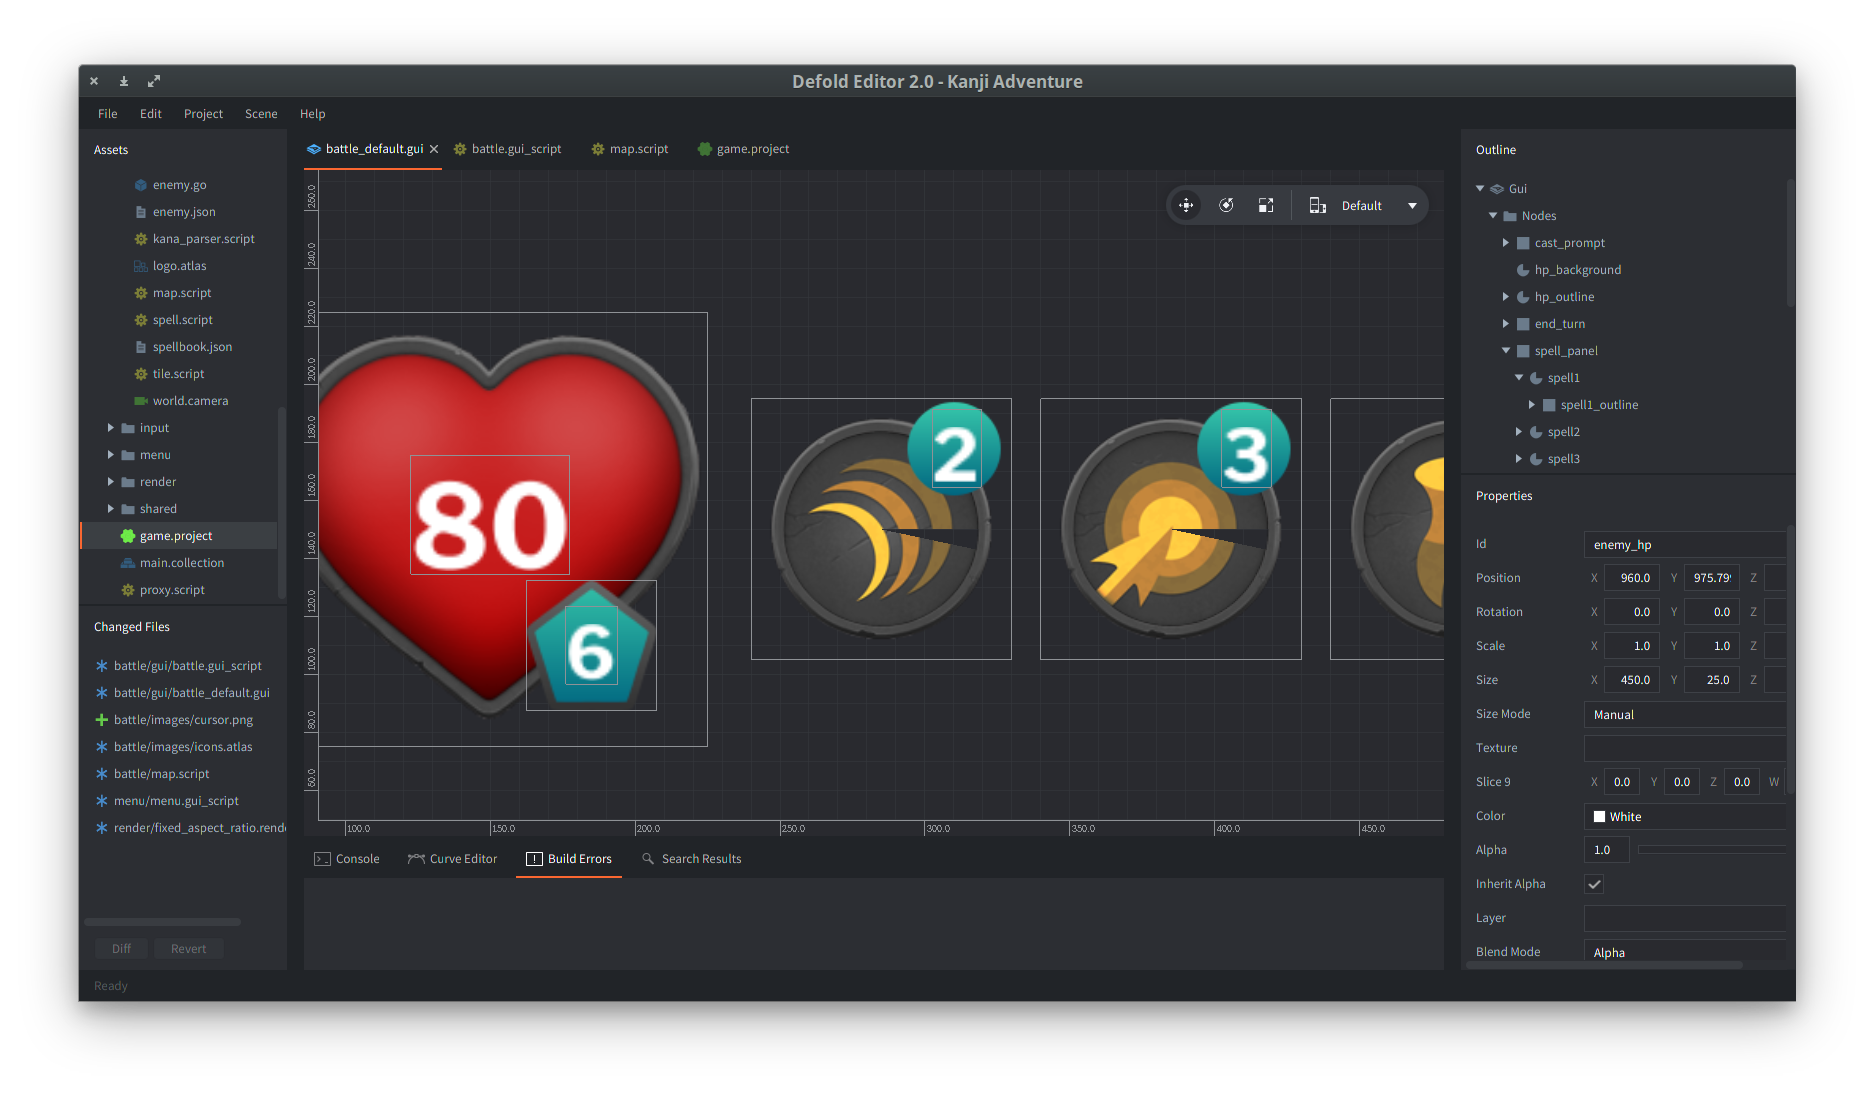
\includegraphics[scale=0.2]{defold}
\caption{Screenshot of Defold's integrated development environment}
\label{fig:defold}
\end{figure}

The other two requirements have been set in order to attempt to hasten the~development process as creating a fully functioning prototype of an~educational RPG by one programmer in approximately four months of time is a rather idealistic goal, especially for someone with no prior game programming experience. These are choosing a tool that includes an intuitive IDE with a fast learning curve as opposed to a bare bones library, and one that is geared specifically towards creating 2D games in order to reduce the need for performance optimization.

\begin{table}[]
\centering
\caption{Comparison of game engines}
\label{engine-comparison}
\scalebox{0.7}{
\begin{tabular}{llllll}
Engine & License & Cost & Targets & Focus & Language\\
Construct 2\autocite{construct} & Proprietary & \$129.99 (\$429.99) & Mobile, (PC, web, Wii U) & 2D & N/A\footnote{Development in Construct 2 is done primarily using a visual event-driven design system. JavaScript is provided as an option.} (JavaScript)\\
Defold\autocite{defold} & Proprietary & free & PC, mobile, web & 2D & Lua\\
Superpowers\autocite{superpowers} & ISC\footnote{Compatible with GNU GPL\autocite{gnuisc}.} & free & PC, mobile, web & 2D, 3D & TypeScript\\
Unity\autocite{unity} & Proprietary & \$0--\$125/mo. & PC, mobile, web, consoles & 2D, 3D & C\#, UnityScript, Boo
\end{tabular}
}
\end{table}

\newpage

We have chosen Defold as the development platform as it allows for targeting all required operating systems --- Windows, macOS, Linux, iOS and Android, features a~\emph{message-driven architecture} that is very easy to comprehend and build around, has an active community and as of early 2017, a brand new IDE. Although console platforms are not officially supported, some console manufacturers include support for HTML5 games via a web applications wrapper, Nintendo Web Framework\autocite{nintendoweb} is one of the examples. It is also geared towards 2D~development, although including 3D assets is possible through slight tweaking of the render script. Defold uses Lua, a lightweight dynamically typed programming language, often used in game development. Defold is also free to use and carries with it no publishing or royalty fees.

The basic building block used in Defold is called a \emph{game object}. Game objects can include scripts that control their behaviour, sprites controlling their visual appearance, factories that can be configured to create other game objects and a variety of other components\autocite{defoldblocks}.

Game objects are grouped inside \emph{collections}, which typically correspond to~scenes used within the game (e.g. main menu, battle, exploration). Communication between objects is handled through a built-in message passing system. Thanks to this system, the programmer seldom has to~use~the~update loop.

\begin{figure}[ht]
\centering
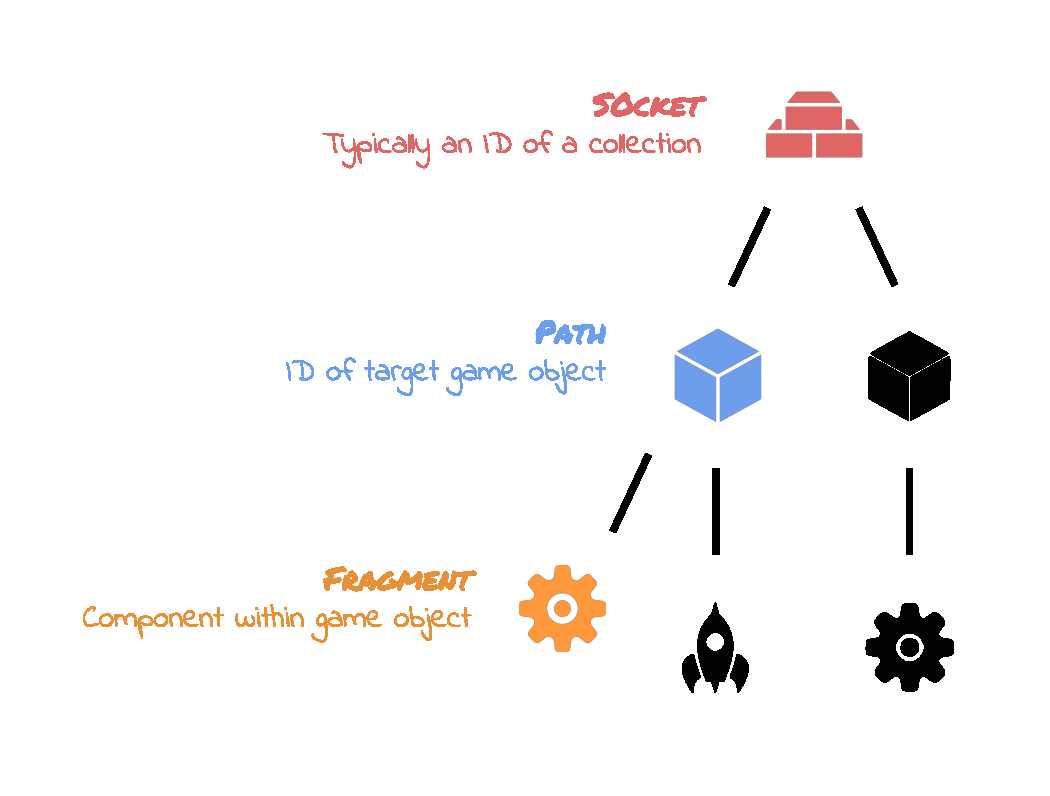
\includegraphics[scale=0.75]{defold_addressing}
\caption{Addressing hierarchy in Defold}
\label{fig:defold_addressing}
\end{figure}

\newpage

The following is an excerpt from code showcasing the messaging system in~action. The target of our message is the `map controller' game object located inside the `battle' collection. The portion behind the hash character names the~component we want to address, in this case a script. The message title is given as the second argument, the third optional argument contains a~Lua~table that includes variables passed as a part of the message\autocite{defoldmessaging}.

\begin{lstlisting}[language={[5.0]Lua}]
msg.post("battle:/map_controller#script","attack_enemy",
        {enemy_number = enemy_num, direction = direction})
\end{lstlisting}

On the receiving end, all we have to do is to add a construct inside the~provided \emph{on\_message} function that resolves the message.

\begin{lstlisting}[language={[5.0]Lua}]
function on_message(self, message_id, m, sender)
  if message_id == hash("attack_enemy") then
    if m.direction == "N" then
      msg.post(self.enemies[m.enemy_number],
               "play_animation", {id = hash("back_attack")})
...
\end{lstlisting}

\section{Tiled Map Editor}

As of May 2017 Defold does not include native support for non-orthogonal tilemaps. Fortunately, there is a number of platform-agnostic map editors available including Tiled\autocite{tiled}, an open-source offering in active development since 2008. It is by far the most popular choice with 2D game creators. We~have chosen this software because it enables creation of \emph{isometric tilemaps}, a~deliberate design choice for our game.

\begin{figure}[ht]
\centering
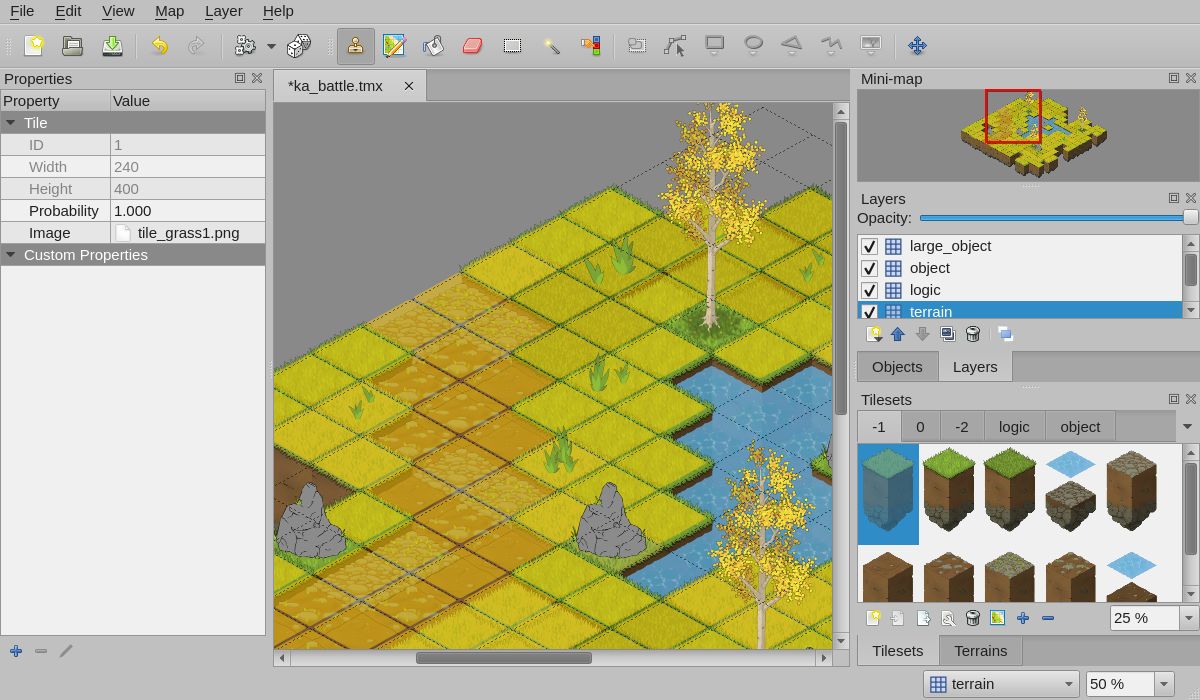
\includegraphics[scale=0.2]{tiled}
\caption{Screenshot of Tiled Map Editor}
\label{fig:tiled}
\end{figure}

The output file includes tile definitions (pairings of image file and its size with a~unique tile id) which are grouped in tilesets, each containing information about offsets and the draw sizes of tiles contained within.

The second part of the output structure includes layer definitions. Each layer has a size, offset from origin and a serialized array which contains placed tiles.

Please keep in mind that the aforementioned contents are in no way an~exhaustive listing of data included in the output file.

\section{Data storage}

There are two commonly used ways to work with external data sources in~Defold, one is to use a Lua table and the other is to utilise the built-in JSON library\autocite{jsonlib}. The developer is free to implement support for other file types using a Lua library or the C++-based native extension system\autocite{nativeext}. As of May 2017 there is no native support for any database engine. One possible workaround could be to run a server-side database with an API endpoint and use Defold's HTTP library\autocite{httplib}, though this process is highly impractical.

\subsection{JSON}

We have chosen JSON as the format of choice for storing most of our data structures due to its easy readability, standardization and built-in support in~Defold. The size of data we store is not as large as to warrant using a~database. Defold supports deserialization of JSON files into Lua tables, however the~reverse process is not possible.

\subsection{Lua table}

The engine allows for serialization and deserialization of tables, a basic Lua data structure. Lua tables are not as human-readable as JSON, therefore we only use them with map files generated by Tiled, which includes Lua support, and save files containing player statistics. In contrast with JSON, Lua tables can be serialized and saved to an external file using built-in library functions.

\section{Git}

Git has been chosen as the version control system for this project due to its integration into Defold IDE's user interface and author's general familiarity with the tool, though it is hardly practical for larger projects.

One issue game developers might encounter while using Git are impracticalities stemming from versioning a large number of sizable binary files that make up the game's assets. The internal `.git' folder can reach large sizes and fetching changes from remote locations can take longer than necessary. Public hosting sites such as GitHub, GitLab and Bitbucket also enforce a size limit on repositories hosted on their sites.

There are two solutions to this problem. One is to use a different VCS such as Subversion, which is better suited to dealing with binary files. The other is~to~utilise what's known as \emph{Git Large File Storage}\autocite{gitlfs}, an open-source tool which replaces large files with pointers to a remote location.

\chapter{Battle system}

\tolerance=1
\emergencystretch=\maxdimen
\hyphenpenalty=10000
\hbadness=10000

\begin{figure}[ht]
\centering
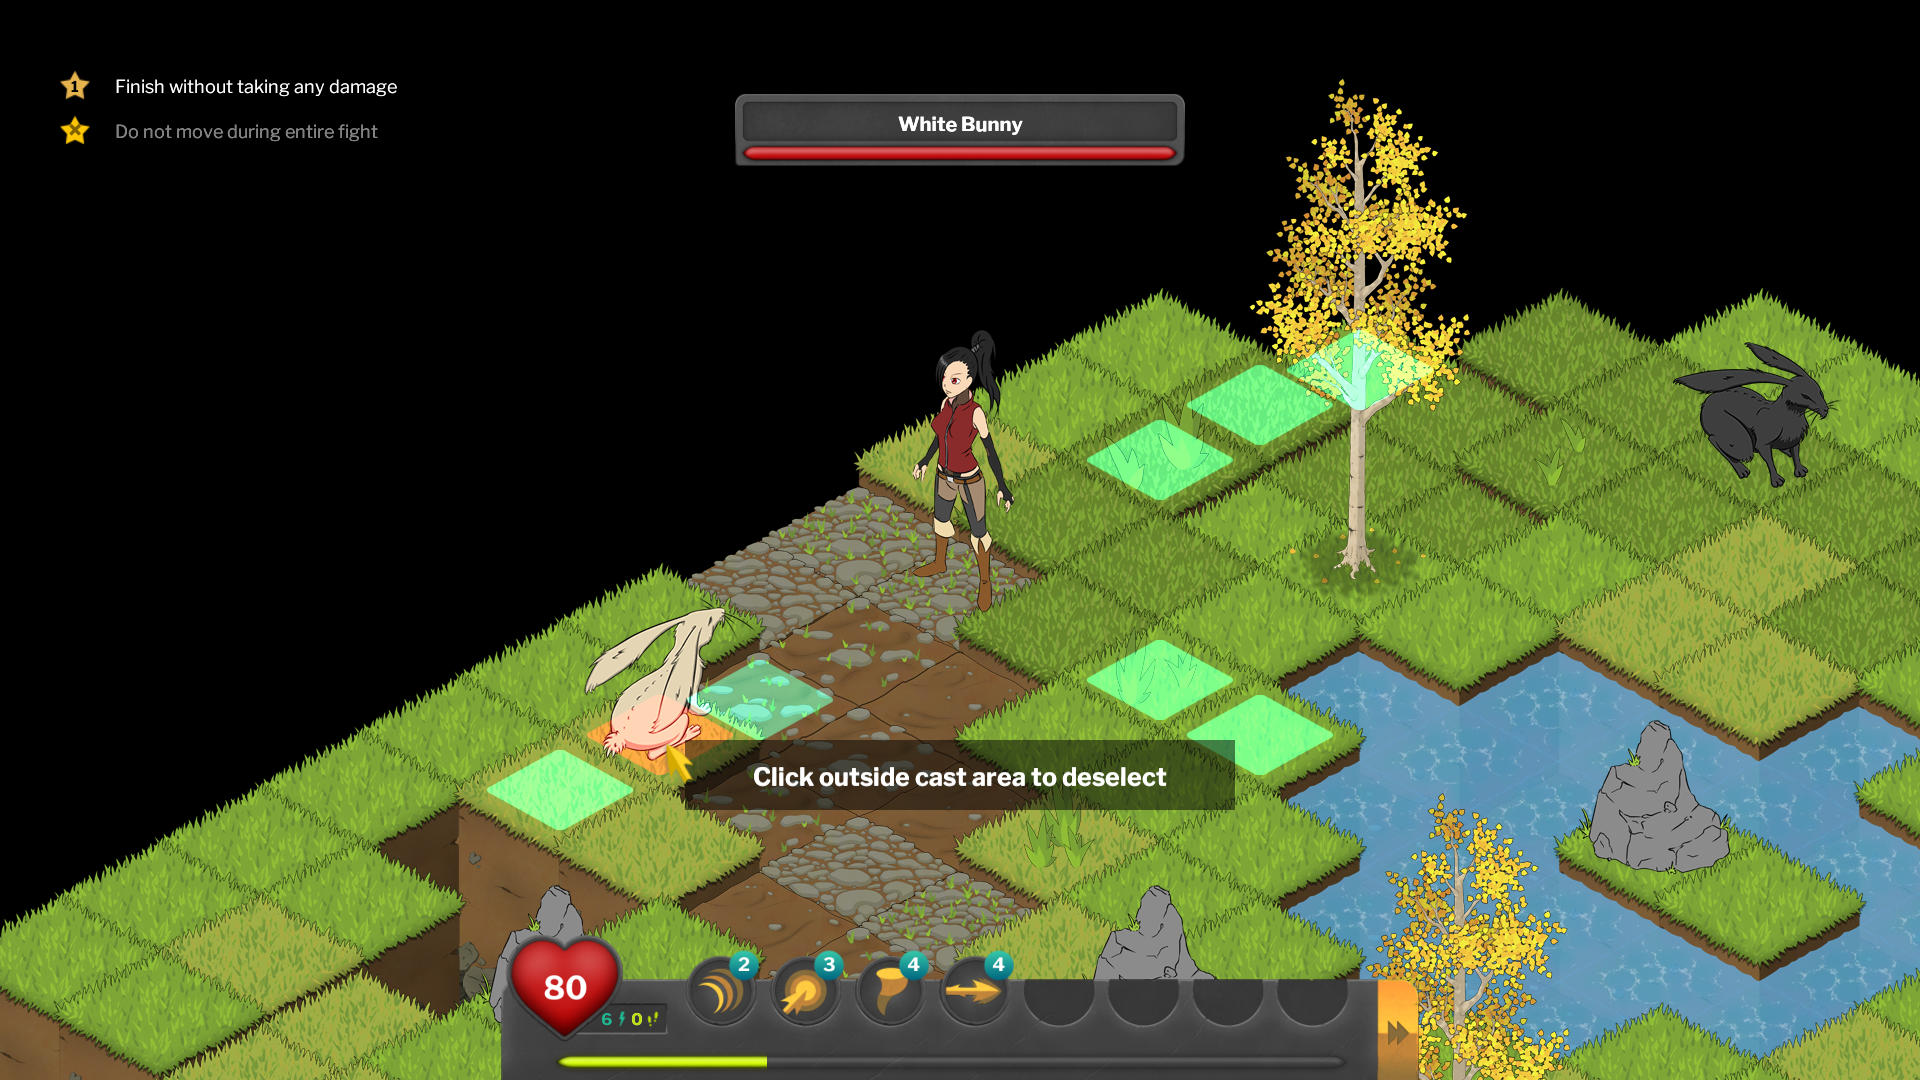
\includegraphics[scale=0.2]{battle}
\caption{In-game screenshot of the battle portion}
\label{fig:battle}
\end{figure}

This chapter includes description of combat mechanics, the learning and the~challenge systems used in the game, a diagram detailing communication between components and a detailed description of these components and data structures exclusive to the battle portion of the game.

\section{Introduction}

The following section details choices made regarding key design elements included within the battle system and the motivations behind these choices.

\subsection{Battle flow}

In the chapter concerning existing products, we have detailed two common approaches used within the turn-based RPG genre. In Fire Emblem and similar JRPGs, during each turn the player moves a character and then performs a~single action, be it using an item, casting a spell or staying still. This approach seems to work best in games that introduce player control over multiple characters. In games with a single controllable character, this approach feels too simplistic and furthermore limits the potential of the game's learning element.

The other mainstream approach is to allow the player to move and cast spells freely during each turn. Utilising this design choice, each spell in the game is given a mana cost that depends on power of the spell. A mana pool of~certain size is refilled at the beginning of each turn and allows the player to~cast multiple spells. Correspondingly the player is allocated a certain number of~movement points that they can utilise during each turn.

\subsection{Learning element}

Each spell has a kanji difficulty setting associated with it that controls which set of phrases is chosen. More powerful spells trigger a choice between more complex kanji phrases.

During the process of choosing phrases for the game, we have decided to divide them into two sets. The first contains kun'yomi readings of characters and therefore includes mostly verbs. The second contains on'yomi readings, which are typically present in kanji compounds. The choice of kanji depends on player character's level and their previous actions. The system \emph{prioritizes kanji} with high error rates.

\newpage

After casting a spell, the player is presented with a \emph{query} containing a kanji character and they are required to type a correct kana transcription. Each spell has a set base damage, which decreases depending on the time it takes to answer the query. We originally planned on introducing an element of~randomness to the amount of damage given, but doing so would negate the~effects of~the~educational element\autocite{lenses}.

\subsection{Challenge system}

The challenge system introduces a set of voluntary \emph{battle-specific goals} that are meant to incentivise certain styles of play in order to alleviate repetition. In contrast with quests, these goals deal exclusively with battle mechanics. Certain challenges are easier than others in order to accommodate skill levels of all players. The implemented examples are as following:

\begin{itemize}
\item Kill an enemy before switching targets.
\item Use a spell at most once a turn.
\item Finish in 10 turns.
\item Finish without taking any damage.
\item Do not fail a single query.
\item Do not move during entire fight.
\end{itemize}

Each challenge is assigned modifiers, which increase the amount of~experience and currency gained on conclusion of the fight should the~challenge be~successfully completed.

\section{Architecture}

\begin{figure}[ht]
\centering
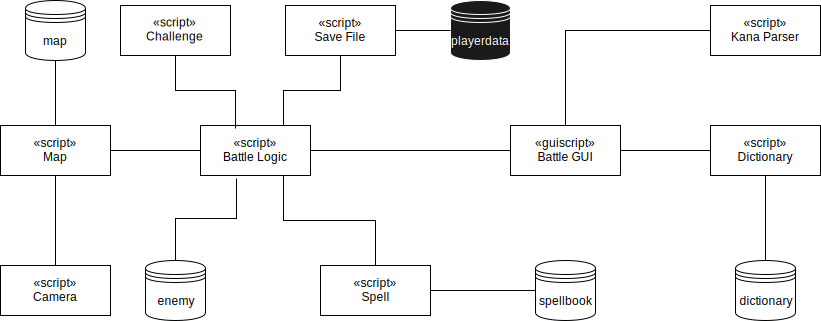
\includegraphics[scale=0.57]{diagram_battle}
\caption{Communications diagram for the game's battle portion}
\label{fig:diagram_battle}
\end{figure}

\subsection{Data structures}

The following section includes details on structures of files used throughout the~battle part of the game. All files are in human-readable JSON format.

\subsubsection{Dictionary}

The file includes two arrays. The first array is used for less powerful spells and includes individual characters, which exclusively use kun'yomi readings, the~second includes more complex composite characters used for~more powerful spells, typically using on'yomi readings. Each entry includes a kanji character or conjugation thereof, its kana transcription and an~English translation.

\begin{lstlisting}
[
    [
        {"kanji": "日", "kana": "ひ", "meaning": "day"},
        {"kanji": "本", "kana": "ほん", "meaning": "book"},
        {"kanji": "人", "kana": "ひと", "meaning": "person"},
        ...
    ],

    [
        {"kanji": "日本", "kana": "にほん", 
         "meaning": "Japan"},
        {"kanji": "日本人", "kana": "にほんじん", 
         "meaning": "Japanese person"},
        ...
    ]
]
\end{lstlisting}

\subsubsection{Spellbook}

The file includes an array of spells used in the game. Each spell has a name, mana cost and a difficulty which corresponds to each of the arrays in dictionary and accepts values of either 1 or 2. Spells have a base damage, which decreases with time used up by player to answer the query, and minimal and maximal ranges indicating distance from player character in number of cells.

Damage range can either be set to 1 which inflicts damage only on~the~selected cell or a larger integer, which also affects a corresponding number of~surrounding cells --- an effect often referred to in video game design as an~\emph{Area~of~Effect} (AoE) spell. The Linear AoE attribute can be set to~1 to make the spell affect targets behind the selected cell (from~player~character's point of view), 2~to inflict damage to targets in-between the~player character and selected cell or~0 to use the more traditional planar AoE.

\begin{lstlisting}
[

    {
        "name": "Whirl",
        "cost": 2,
        "kanji_difficulty": 1,
        "base_damage": 45,
        "min_range": 1,
        "max_range": 1,
        "damage_range": 1,
        "linear_aoe": 0
    },
    ...
]
\end{lstlisting}

\newpage

\subsection{Script entities}

The following section contains information about script entities used in~the~battle part of the game.

\subsubsection{Battle logic}

Controls the flow of a battle. Structures included within control movement, actions and statistics of both the player character and any enemies present on~the~map. \emph{A* search algorithm}\autocite{astar} is used to find the shortest paths for both the~enemies and the player to follow. Validity of cells in regards to movement and casting is determined by the map's logic layer.

\subsubsection{Battle GUI}

Updates information present on the game's user interface. The script also manages all keyboard and mouse/touch input from the player when a battle is ongoing.

\subsubsection{Dictionary}

This script is utilized during the process of casting a spell. It chooses a kanji with the lowest success rate from the dictionary data structure to use during a~query. After completion of the query, it saves the result to a save file.

\subsubsection{Challenge}

Picks two random entries from the list of available challenges and afterwards keeps track of their status (in progress, successfully completed, failed). Due to~the~need to incorporate hooks into other scripts, the challenge list is~hard~coded and therefore doesn't depend on an external data structure.

\subsubsection{Spell}

Determines valid targets during the spell casting process based on information present in the spellbook data structure and logic layer of the current map. Also calculates damage based on time taken by the player to answer a query and base damage of the selected spell.

\newpage

\subsubsection{Kana parser}

Works in conjunction with battle GUI to translate Latin characters written by the player into hiragana. The parser adheres to rules defined by \emph{Hepburn romanization system}, the most widely used transcription method. The solution for more complex cases, such as the insertion of small `sokuon' characters is inspired by the behaviour of Microsoft Input Method Editor for Japanese.

\begin{table}[htb]
\centering
\caption{Hiragana conversion table}
\label{hiragana-table}
\begin{tabular}{lllllllll}
 & a & i & u & e & o & ya & yu & yo\\
ー & あ & い & う & え & お & や & ゆ & よ\\
k & か & き & く & け & こ & きゃ & きゅ & きょ\\
s & さ & ー & す & せ & そ & ー & ー & ー\\
t & た & ー & ー & て & と & ー & ー & ー\\
n & な & に & ぬ & ね & の & にゃ & にゅ & にょ\\
h & は & ひ & ー & へ & ほ & ひゃ & ひゅ & ひょ\\
m & ま & み & む & め & も & みゃ & みゅ & みょ\\
y & や & ー & ゆ & ー & よ & ー & ー & ー\\
r & ら & り & る & れ & ろ & りゃ & りゅ & りょ\\
w & わ & ー & ー & ー & を & ー & ー & ー\\
g & が & ぎ & ぐ & げ & ご & ぎゃ & ぎゅ & ぎょ\\
z & ざ & ー & ず & ぜ & ぞ & ー & ー & ー\\
d & だ & ー & ー & で & ど & ー & ー & ー\\
b & ば & び & ぶ & べ & ぼ & びゃ & びゅ & びょ\\
p & ぱ & ぴ & ぷ & ぺ & ぽ & ぴゃ & ぴゅ & ぴょ
\end{tabular}
\end{table}

\begin{table}[htb]
\centering
\caption{Special cases of hiragana conversion}
\label{hiragana-table-special}
\begin{tabular}{llllll}
Romaji & Kana & Romaji & Kana & Romaji & Kana\\
n & ん & fu & ふ & shi & し\\
sha & しゃ & shu & しゅ & sho & しょ\\
chi & ち & tsu & つ & cha & ちゃ\\
chu & ちゅ & cho & ちょ & ji & じ\\
ja & じゃ & ju & じゅ & jo & じょ
\end{tabular}
\end{table}

\newpage

\begin{figure}[ht]
\centering
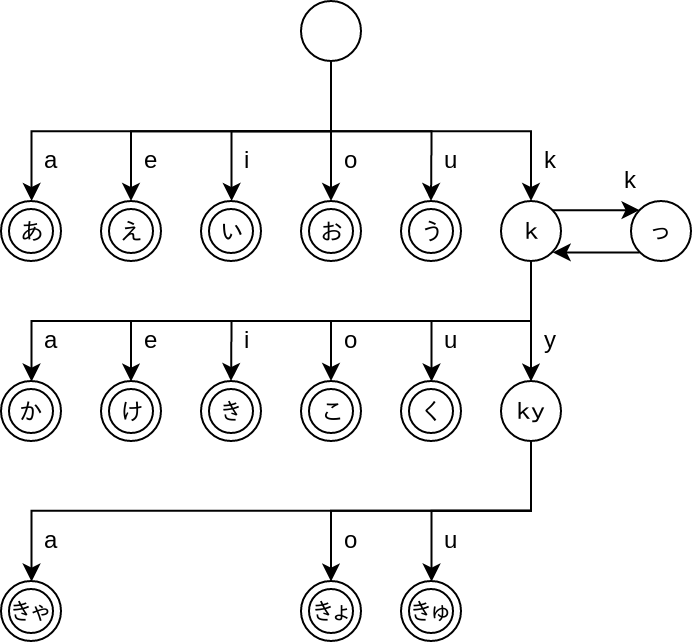
\includegraphics[scale=1]{kana_parser}
\caption{Simplified finite-state automaton for the first two rows of the hiragana conversion table}
\label{fig:kana_parser}
\end{figure}

\chapter{Exploration system}

\tolerance=1
\emergencystretch=\maxdimen
\hyphenpenalty=10000
\hbadness=10000

\begin{figure}[ht]
\centering
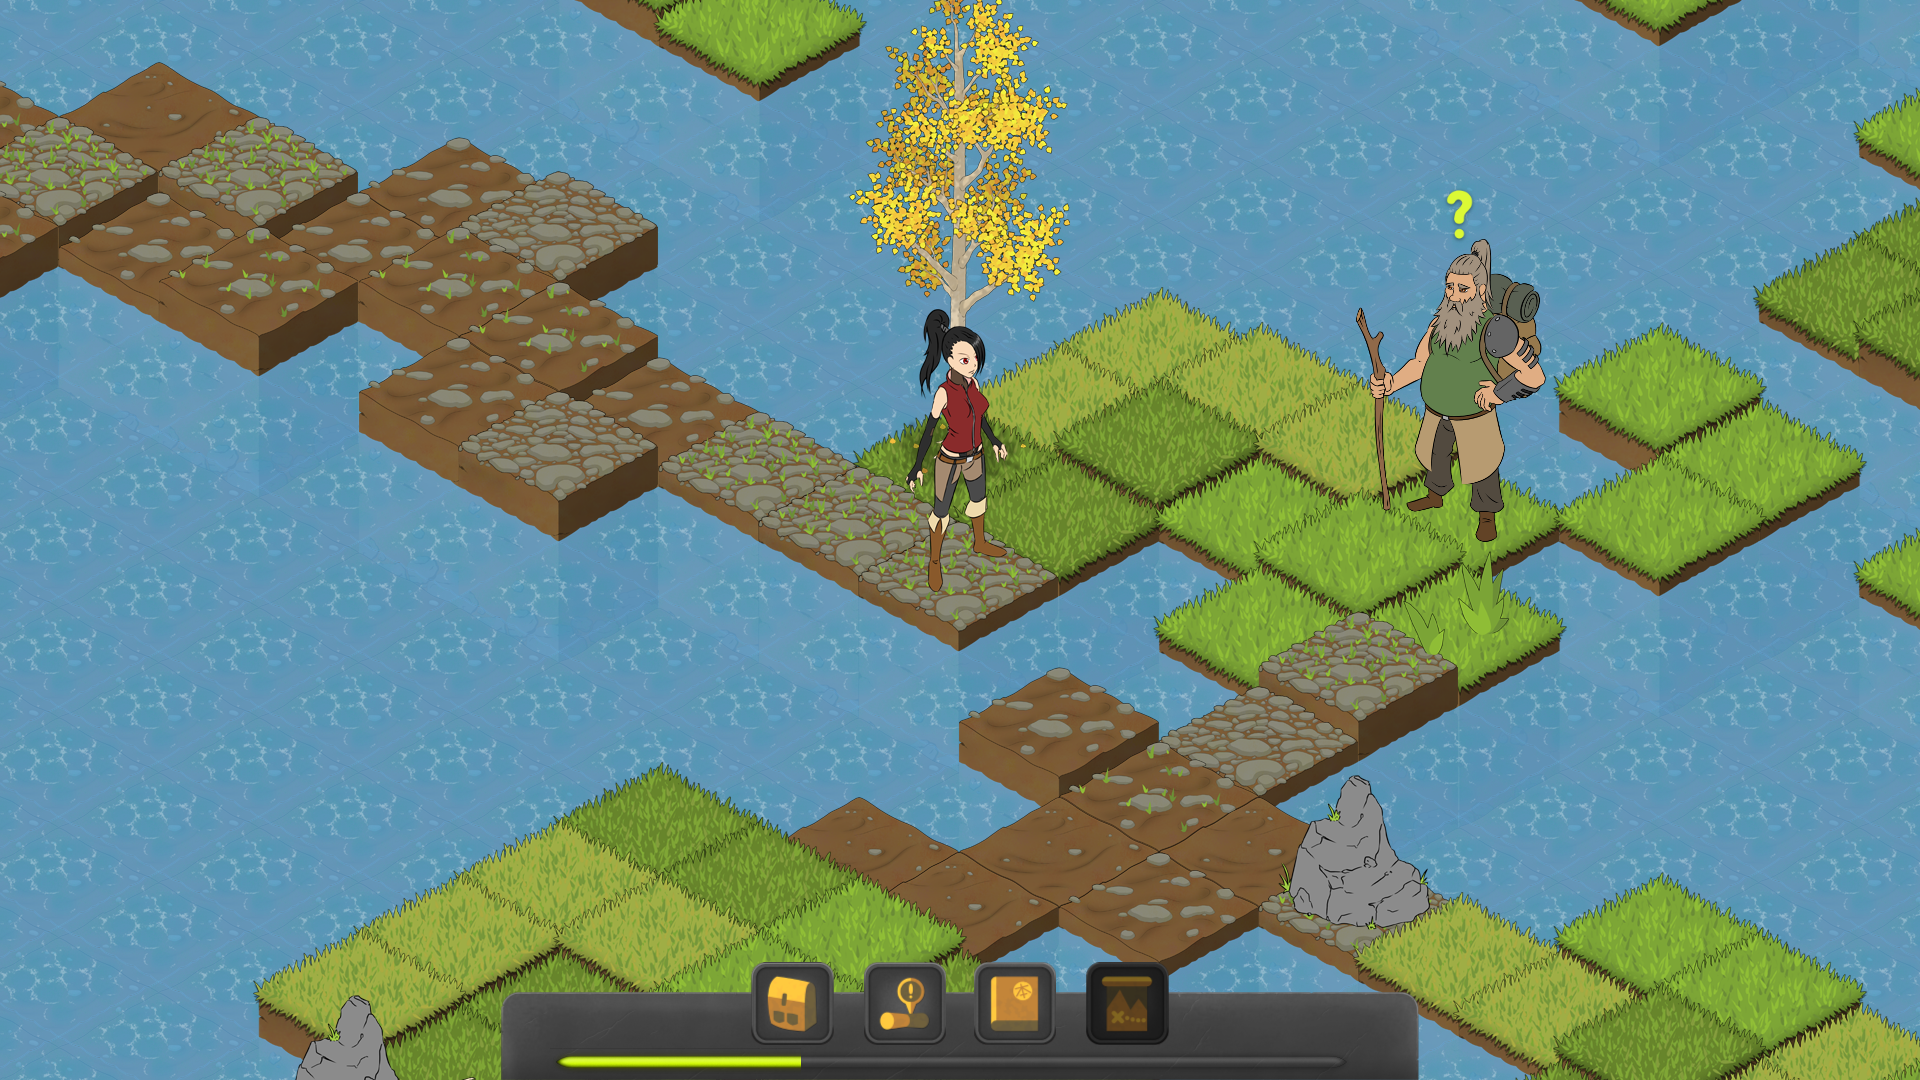
\includegraphics[scale=0.2]{explore}
\caption{In-game screenshot of the exploration portion}
\label{fig:explore}
\end{figure}

This chapter details the questing system used within our game, introduces the~item system and item economy and talks about the experience system. As~with~the~battle chapter, we discuss data structures and script components exclusive to this part of the game.

\section{Introduction}

The following section details choices made regarding key design elements included within the exploration system and the motivations behind these choices.

\subsection{Questing system}

The quest system is an \emph{important plot device} that motivates the player and helps alleviate the negative effects of grind mechanics on player retention. While researching the possible quest archetypes, we wanted to focus on three aspects --- repeatability, quests as means of motivating the player to move between game areas and variability.

\subsubsection{Repeatability}

The first aspect concerns quests that are meant to be experienced multiple times. Repeatable quests entice the player to return to previous areas and usually provide rewards that are exclusive to the particular region of the map they take place in.

\subsubsection{Exploration quests}

These quests are generally one-time-only opportunities that are designed to~move the~player from one area to another in a smooth and believable fashion. These types of quests are utilised in World of Warcraft, where they are colloquially referred to as \emph{breadcrumb quests}. We will work with branching quest arcs, however, for the sake of simplicity, no two quests can be mutually exclusive.

The following diagram illustrates the relationships between quests. Black exclamation marks symbolise main quests, while light gray marks symbolise side quests. Main quests are dependent on one another, while side quests are optional. Many main quests are of the breadcrumb type, as discussed in~the~previous paragraph, though this is not always the case.

\begin{figure}[ht]
\centering
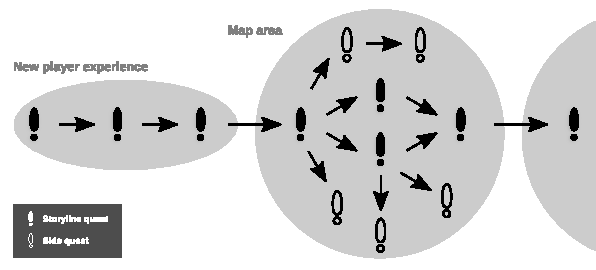
\includegraphics[scale=1.3]{diagram_quests}
\caption{Quests diagram}
\label{fig:diagram_quests}
\end{figure}

\subsubsection{Variability}

One issue a lot of modern role-playing games face is the lack of variability when it comes to quests. The player is generally asked to kill a certain number of enemies or to collect certain items. To help combat this fact, we have listed below some examples that can be used within our game:

\begin{itemize}
\item character hunting quest (triggering conversations with different NPCs),
\item scavenger hunt (locating certain cues hidden within the environment),
\item enemy killing quest (killing a number of enemies of a specific type),
\item gathering quest (collecting a number of resources from enemies or~crafting nodes),
\item achievement quest (meeting a condition, such as achieving consistent success in regards to the learning element or completing a~number~of~challenges).
\end{itemize}

\newpage

\subsection{Item system}

The game has three categories of items. Equipment, which the player can wear to change the behaviour of certain parts of the game, consumables that they can use in battle to increase health and potentially cause other effects, and resources, which are used for completing quests or can be further refined via~crafting.

\subsubsection{Equipment}

Equipment in most modern role-playing games is designed to increase player statistics. As a player, I feel this approach is rather artificial and lacking. Besides, in an educational game, focus should be given on the~educational element. The proficiency of the player should be the main factor in determining their potency.

Therefore, we have designed the equipment to \emph{alter game mechanics} in ways that both benefit and punish the player in certain areas, a mechanic similar to~the~idol system in Dofus. For example, certain players might prefer to have more time when answering queries. They can wear an item that increases available time, but decreases damage that the spell causes. Other players could prefer the opposite, so another item will exist which decreases available time and increases damage caused, thus rewarding players with faster memory recall skills.

\subsubsection{Consumables}

Consumable items are meant to be used within the game's battle mode. They generally provide additional health points to the player and can be essential for more difficult fights. They can also provide \emph{supplementary effects} such as temporary stuns, increase available movement points and more. No~consumables should provide damage dealing capabilities as doing so would interfere with spells and the associated learning element. When using a~consumable, the player does not have to answer a query.

\subsubsection{Resources}

The resources category contains items that can be used to create consumables, used in gathering quests, or do not perform any function other than \emph{generating profit} for the player via the mechanic of selling the item to the vendor NPC.

\subsection{Economy}

Activities that bring items into economy are called item fountains (or faucets, depending on literature), activities that remove items from the game's economy are called item sinks. Balancing the two is a vital part of~role-playing game design.

Designing item fountains is a fairly straightforward process. In our game, there are presently two such examples --- winning an item in combat and acquiring it as a quest reward.

Creating item sinks is a comparatively more difficult process. Examples of~item sinks used in RPGs today include maintenance fee, where an item will lose its effect unless some amount of currency is paid periodically, limited inventory space (and to a lesser degree a weight system), where the player needs to discard an old item in order to acquire a new one, or a crafting system, which lets players exchange a combination of items for a new item\autocite{economies}.

In our game we have designed three item sinks. Consumable items can be~used during battle to heal the player and perform additional effects. Certain resource items are utilised in quests. Last but not least, items can be traded to a~vendor NPC in exchange for currency (not pictured in the diagram for~the~sake~of~visual~clarity).

Future implementation of a crafting system will introduce an additional item~fountain --- \emph{the gathering node}. Additionally, the process of crafting itself is~both an~item fountain and an item sink.

\newpage

\begin{figure}[htb]
\centering
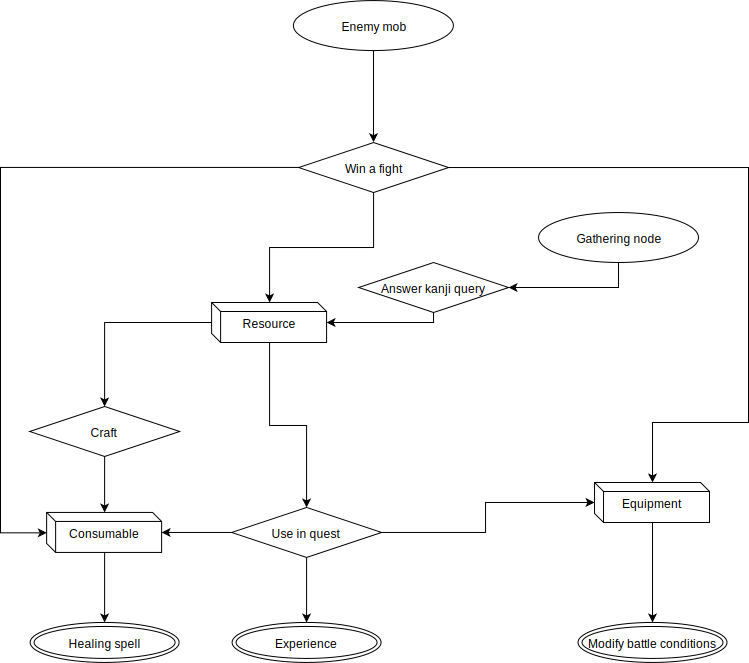
\includegraphics[scale=0.6]{item_economy}
\caption{Economy diagram}
\label{fig:item_economy}
\end{figure}

\subsection{Learning progression}

As hinted in previous chapters, the game includes an experience system. Most role-playing games use this system to lock players out of content that is~meant to be experienced in later stages of the game. They do this by introducing statistics, which increase with level or by specifying level requirements for equipment. When designing the game, we wanted to stay away as much as possible from arbitrary numbers that influence the might of~player's character and instead let the strategy and most importantly knowledge of kanji characters determine player's success.

On the other hand, we needed a system that adds new kanji characters to~the~pool of phrases that are used in the battle system. The solution is~simple --- when the player gains a new level, they unlock a new kanji character.

\section{Architecture}

\begin{figure}[ht]
\centering
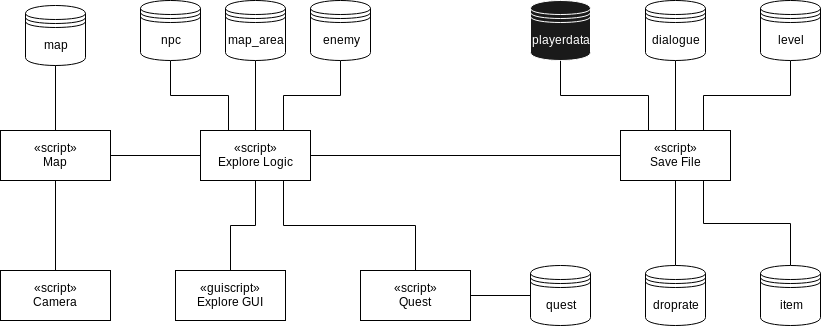
\includegraphics[scale=0.57]{diagram_explore}
\caption{Communications diagram for the game's exploration portion}
\label{fig:diagram_explore}
\end{figure}

\subsection{Data structures}

The following section includes details on structures of files used throughout the exploration part of the game. All files are in human-readable JSON format.

\subsubsection{Item}

This structure holds data on all items within the game. Each item entry contains an identifier, a name, filename for its inventory icon, value when sold to~the~vendor NPC, the category definition and effects of the item when used by the player, which are applicable for items from equipment and consumable categories. Equipable items include information about slot that they occupy on~the~player character. Additionally, a description is provided that displays inside GUI tooltips when hovering over the item in question.

\begin{lstlisting}
[

    {
        "id": 15,
        "name": "Ring of life",
        "icon": "life_ring",
        "description": "A ring with an integrated defibrilation unit.\n+15 health points\n-20% damage given",
        "value": 0,
        "category": "equipment",
        "slot": "accessory",
        "effects": {
            "health": 15,
            "damage_given": -0.2
        }
    },
    ...
]
\end{lstlisting}

\subsubsection{Droprate}

This structure is used when determining spoils of battle. Each entry represents an enemy. In addition to the enemy identifier, it contains a nested array of~items obtainable from winning a battle against that enemy. Each entry in~this nested array contains an item identifier and a probability value, which is a~positive number that determines the probability of dropping the item in~decimal fractions. The currency value determines the maximum amount of~in-game currency attainable by defeating a single enemy. The resulting amount ranges from 60 to 100 percent.

\begin{lstlisting}
[

    {
        "enemy_id": 1,
        "currency": 5,
        "items": [
            {
                "item_id": 1,
                "probability": 0.3
            },
            {
                "item_id": 3,
                "probability": 0.7
            }
        ]
    },
    ...
]
\end{lstlisting}

\subsubsection{NPC}

The structures includes information on non-playable characters. Each entry includes an identifier, a name of the character which is displayed in dialogues, name of the animation that represents the character, position within the game world specified by the map area and position coordinates, a flag which specifies whether the NPC functions as a vendor and an initial dialogue that is added to~a~new save file at the start of the game.

\begin{lstlisting}
[

    {
        "id": 1,
        "name": "Old Guy",
        "sprite": "npc_man",
        "map_area": 1,
        "position": [12, 24],
        "vendor": false,
        "starting_dialogue": 25
    }
    ...
]
\end{lstlisting}

\subsubsection{Dialogue}

Dialogues in the game are ordered in a linear fashion. There are no instances of~branching dialogues. Each dialogue entry contains an identifier, the dialogue text itself and an identifier of the follow-up dialogue, if applicable.

\begin{lstlisting}
[

    {
        "id": 2,
        "text": "Hello there stranger, I haven't seen a fresh soul as of late. You seem to be new around these parts, am I right? Well then... *ahem* let me introduce you to...",
        "next_dialogue": 3
    },
    ...
]
\end{lstlisting}

\subsubsection{Quest}

This structure contains information on quests. Each entry contains an identifier, identifiers of both the NPC that gives the quest to the player and the one that gives the reward for a finished quest, the dialogues that are triggered when the~quest is available and completed respectively, flags that hold information on~whether the quest is repeatable and whether it is a quest from the main storyline (these are displayed in the GUI with a different icon), the title of~the~quest and description visible in the quest GUI, a prerequisites array that holds identifiers of quests that need to be completed before the quest in~question becomes available, triggers that specify player actions required to~complete the~quest (as with challenges these are hard coded) and information about rewards in~experience, currency and items.

\begin{lstlisting}
[

    {
        "id": 1,
        "start_npc": 1,
        "end_npc": 1,
        "repeatable": false,
        "story": true,
        "title": "Into the fray",
        "description": "The old man wants you to defeat a rabbit to prove your worth. You aren't going to let him down, are you?",
        "prerequisites": [],
        "triggers": [["KILL_ENEMY", 1, 1]],
        "exp_reward": 500,
        "currency_reward": 60,
        "item_reward": [1, 1, 5],
        "start_npc_dialogue": 2,
        "end_npc_dialogue": 6
    }
    ...
]
\end{lstlisting}

\newpage

\subsubsection{Map area}

This structure includes the name of each area, map file used, list of items sold by~vendors in the area and their costs and information about enemy mobs. Every mob has a position associated with it, the enemies respawn at~the specified location on map load and then proceed to wander about. The~level~designer has an option to specify the number of enemies and their type for each mob in the `enemies' array. This information is not required, if it is not provided, the map loading routine will generate a random assortment of enemies that can be controlled using the `enemy\_types' array and the~`max\_mob\_size' field. The~former contains nested arrays, which specify enemy id and spawn probability. The sum of probabilities can be any positive number. The `max\_mob\_size' field allows for choosing the maximum mob size as generated mobs differ in number of enemies.

\begin{lstlisting}
[

    {
        "id": 1,
        "name": "Rabbit Island",
        "map_file": "ka_rabbit",
        "enemy_types": [[1, 0.2], [2, 0.1]],
        "max_mob_size": 4,
        "enemy_mobs": [
            {
                "enemies": [1],
                "position": [30, 66]
            },
            {
                "enemies": [3, 2, 2, 1],
                "position": [66, 22]
            },
            {
                "position": [38, 27]
            },
 		    {
                "position": [36, 19]
            },
 	        ...
        ],
        "vendor_items": [
            {
                "item": 4,
                "cost": 400
            },
            ...
        ]
    }
    ...
]
\end{lstlisting}

\subsection{Script entities}

The following section contains information about script entities used within the exploration part of the game.

\subsubsection{Explore logic}

Controls the flow of the out-of-battle mechanics. Structures included within control movement and actions of the player character and both enemies and NPCs present on the map. A* search algorithm is used to find the shortest paths for the player to follow, enemies move randomly to unoccupied neighboring tiles. Validity of cells in regards to movement is determined based on~the~map's logic layer.

\subsubsection{Explore GUI}

Updates information present on the game's user interface. The script also manages all keyboard and mouse/touch input from the player when out~of~battle. Due to complicated UI elements, the GUI is divided between four files --- inventory, encyclopaedia and quest GUIs and the explore GUI file, which includes links to the remaining three files via built-in template functionality. Unfortunately, Defold does not allow the developer to add separate GUI scripts to linked GUI files\autocite{defoldtemplate}.

\newpage

\subsubsection{Quest}

The script handles operations concerning quests. Receives updates on triggers and propagates them into the persistence module. Checks on quest status and passes on information about quest markers that display atop NPCs to~the~map~script, and general quest information to the explore GUI script to~be~displayed in~relevant GUI elements. As with the challenge script in~the~battle portion, triggers are hard coded due to the need to incorporate hooks into~other~scripts.

There are 5 states a quest can be in. By default, it is \emph{inactive} and therefore unavailable to the player. After prerequisites are met, the quest enters the~\emph{available} state and is available for the player to accept. The quest-giving NPC displays an exclamation mark on top of their sprite. Once the quest is accepted by the player, it enters the \emph{ongoing} state. The quest script then looks for triggers associated with the quest. Once conditions of all triggers in the~quest have been met, the quest enters the \emph{turn-in} state. In this state, the~quest-ending NPC displays a question mark on top of their sprite and the~player is able to turn in their quest and claim their reward, after which the~quest enters the \emph{completed} state, unless it is a repeatable quest, in which case we return the~quest to~its~\emph{available} state.

The following list includes all triggers that are currently implemented:

\begin{itemize}
\item Defeat a certain number of enemies.
\item Complete a certain number of challenges.
\item Obtain a certain number of items.
\item Collect a certain number of kanji tablets\footnote{Kanji tablets are a metaphor used to represent levels.}.
\item Collect a certain number of trinkets\footnote{Trinkets are items with a physical representation on the game map.}.
\end{itemize}

\chapter{Shared elements}

\tolerance=1
\emergencystretch=\maxdimen
\hyphenpenalty=10000
\hbadness=10000

This chapter contains information on data structures and script components used outside of and in both the battle and exploration parts of the game. Additionally, it details the persistence module and the used tile rendering algorithm.

\section{Introduction}

\subsection{Persistence module}

The persistence module stores all \emph{non-static information} and changes dynamically depending on player's actions. It also handles initialisation in~the~case of player starting a new game. Changes are saved often as to meet our functional requirement concerning short gameplay sessions.

\subsection{Tile rendering}

As we do not use Defold's built-in tile editor, we had to write our own routine for rendering tiles. Due to the large size of maps used within the exploration mode, rendering all the tiles at once would use up a significant amount of~system resources.

\newpage

For example, a map with a size of 100 by 100 tiles would require the engine to~store 30,000 sprites (each tile collection includes three game objects and in~turn sprites associated with it --- the terrain, object and a~selection image). To~optimise the performance, we have to render only tiles that are visible within the current camera view.

There are two programmatic approaches we can use to implement \emph{dynamic tile rendering}. One is to remove game object instances that are no longer visible and add new instances. The other is to keep the existing game objects and move them from their original position to the new position. The practice of reusing intialised objects is called object pooling. It is used to mitigate performance issues when dealing with objects whose initialisation and destruction routines are resource intensive. Defold already has object pooling implemented on an engine level and the documentation specifically advises developers to use the earlier approach\autocite{defoldpooling}.

The developer can also decide on whether to complete the entire operation at~once or whether to divide the process into steps that line up with character movement.

While trying both approaches, we have come across a large difference in~performance, although on further inspection we found out it was due to lack of~optimisation on our part. We used to unnecessarily iterate through structural metadata about tilesets while preparing every single tile. We~managed to solve this issue by creating a Lua table that stores tileset data about every tile style used.

\newpage

\section{Architecture}

\subsection{Data structures}

The following section includes details on structures of files used throughout the entirety of the game. Both the map files and the persistence module are stored inside files containing Lua tables. The level and enemy data structures are stored in JSON files.

\subsubsection{Persistence module}

The persistence module acts as a save file. It contains data on player's success rate for each kanji phrase, entries on active and completed quests, current NPC dialogues, items located in player's inventory and equipped on their character, balance of in-game currency, their level and experience points, which determine the size of the kanji selection pool.

\subsubsection{Map}

Maps are stored in a Lua script file. Tiled export formats also include JSON and CSV. For a brief summary of contents, please refer to the Technology section of this thesis. As of version 0.17 Tiled also supports Defold's native tile format, however the current implementation only allows for orthogonal maps and is therefore unsuitable for our game.

The game uses four map layers to store data:

\begin{enumerate}
\item large\_object --- contains sprites spanning multiple tiles (e.g. trees),
\item object --- contains smaller obstacles such as rocks or tile decorations,
\item logic --- used by the battle logic script to determine whether a cell is~accessible,
\item terrain --- contains base tiles.
\end{enumerate}

\subsubsection{Enemy}

The file includes information about all enemies in the game. Each enemy entry contains a type definition used internally within the game, name displayed as part of battle GUI, initial health value, number of moves, base~damage, attack~range and number of experience points awarded to~the~player for~a~successful kill.

\begin{lstlisting}
[

    {
        "id": 1,
        "type": "white_bunny",
        "name": "White Bunny",
        "health": 60,
        "movement_pool": 3,
        "attack": 6,
        "range": 1,
        "experience": 30
    },
...
]
\end{lstlisting}

\newpage

\subsubsection{Level}

The file contains information on player levels and query phrases associated with them. Levels have an experience value associated with them. When a player gains a specified amount of experience, they reach a new level and unlock a new kanji character. This process widens the number of possible queries by adding phrases that contain the character. The `basic' and `complex' fields indicate the~position of the last phrase that can be shown to the player of that particular level. They correspond to the first and second arrays of the dictionary data structure. Information on kun'yomi and on'yomi readings are also included for~the~encyclopedia GUI to make use of.

\begin{lstlisting}
[

    {
        "kanji": "日",
        "kun": "ひ",
        "on": "にち",
        "basic": 1,
        "complex": 0,
        "experience": 100
    },
    ...
]
\end{lstlisting}

\newpage

\subsection{Script entities}

The following section contains information about script entities used in both the battle and exploration parts of the game.

\subsubsection{Save file}

Retrieves data from and saves data to player's save file. Handles initialisation of new save files with default values.

\subsubsection{Proxy}

Collection proxies in Defold handle loading and unloading collections, structures that contain game objects and can be often thought of as scenes of~the~game. The proxy script handles switching between the menu, battle and exploration parts of the game, allocating system resources as needed.

\subsubsection{Menu GUI}

Includes input handling for buttons in the game menu.

\subsubsection{Tutorial GUI}

Controls display of tutorial images.

\subsubsection{Render script}

The game includes an implementation of a render script that maintains fixed aspect ratio made by Defold developer Björn Ritzl\autocite{britzl}.

\subsubsection{Map}

Renders terrain tiles, objects and characters in a correct order based on~information included within the map data structure as well as parameters passed from outside scripts.

\newpage

The script also handles conversion between input coordinates and the game's coordinate system. Map coordinates are calculated using the following transformation matrix:

\[
\frac{1}{2wh} 
\begin{pmatrix}
h & w & -f_{x}h - f_{y}w \\
-h & w & f_{x}h - f_{y}w \\
0 & 0 & 2wh
\end{pmatrix}
\]

In this matrix, $w$ and $h$ refer to width and height of a tile in pixels respectively and $f_{x}$ and $f_{y}$ refer to offsets of origin in both dimensions\autocite{sojka}.

\subsubsection{Camera}

Moves the camera game object in a smooth fashion using linear interpolation with variable speed. We have decided on keeping the camera permanently locked on the location of the player character. Originally, the camera moved to~the~target location in a straight line, but doing so presents a problem in~specific environments, such as the one pictured below. If player were to move between the two points pictured, the player character would move off-screen, stay invisible for a couple seconds and then re-appear, which could potentially confuse the player.

\begin{figure}[ht]
\centering
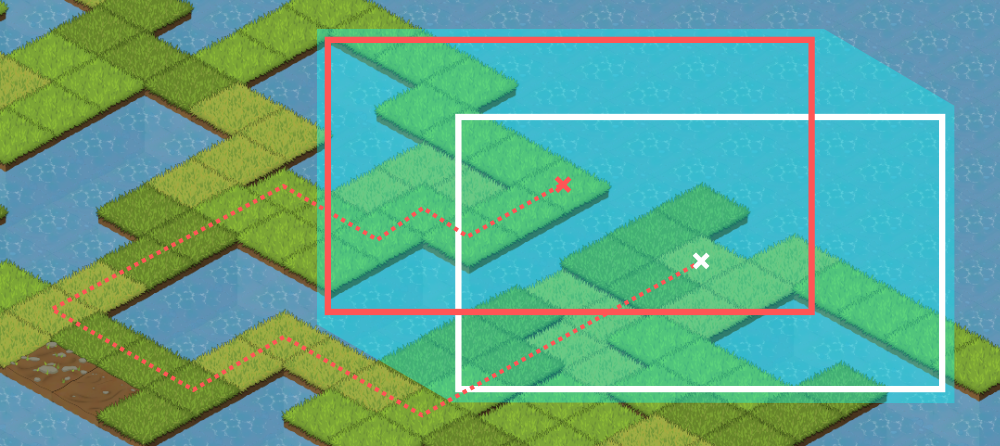
\includegraphics[scale=1]{camera_change}
\caption{Illustration showcasing issue with camera movement}
\label{fig:camera_change}
\end{figure}

\chapter{Tutorial}

\tolerance=1
\emergencystretch=\maxdimen
\hyphenpenalty=10000
\hbadness=10000

This chapter details the process of introducing the player to key gameplay mechanics via a series of images that guide the player to perform specific actions. This approach was chosen for its ability to immerse the player into~the~game. We wanted to avoid using complex pop-up dialogues as they detract from the experience. The comparatively small window on top right can~be easily ignored if wanted to.

\begin{figure}[ht]
\centering
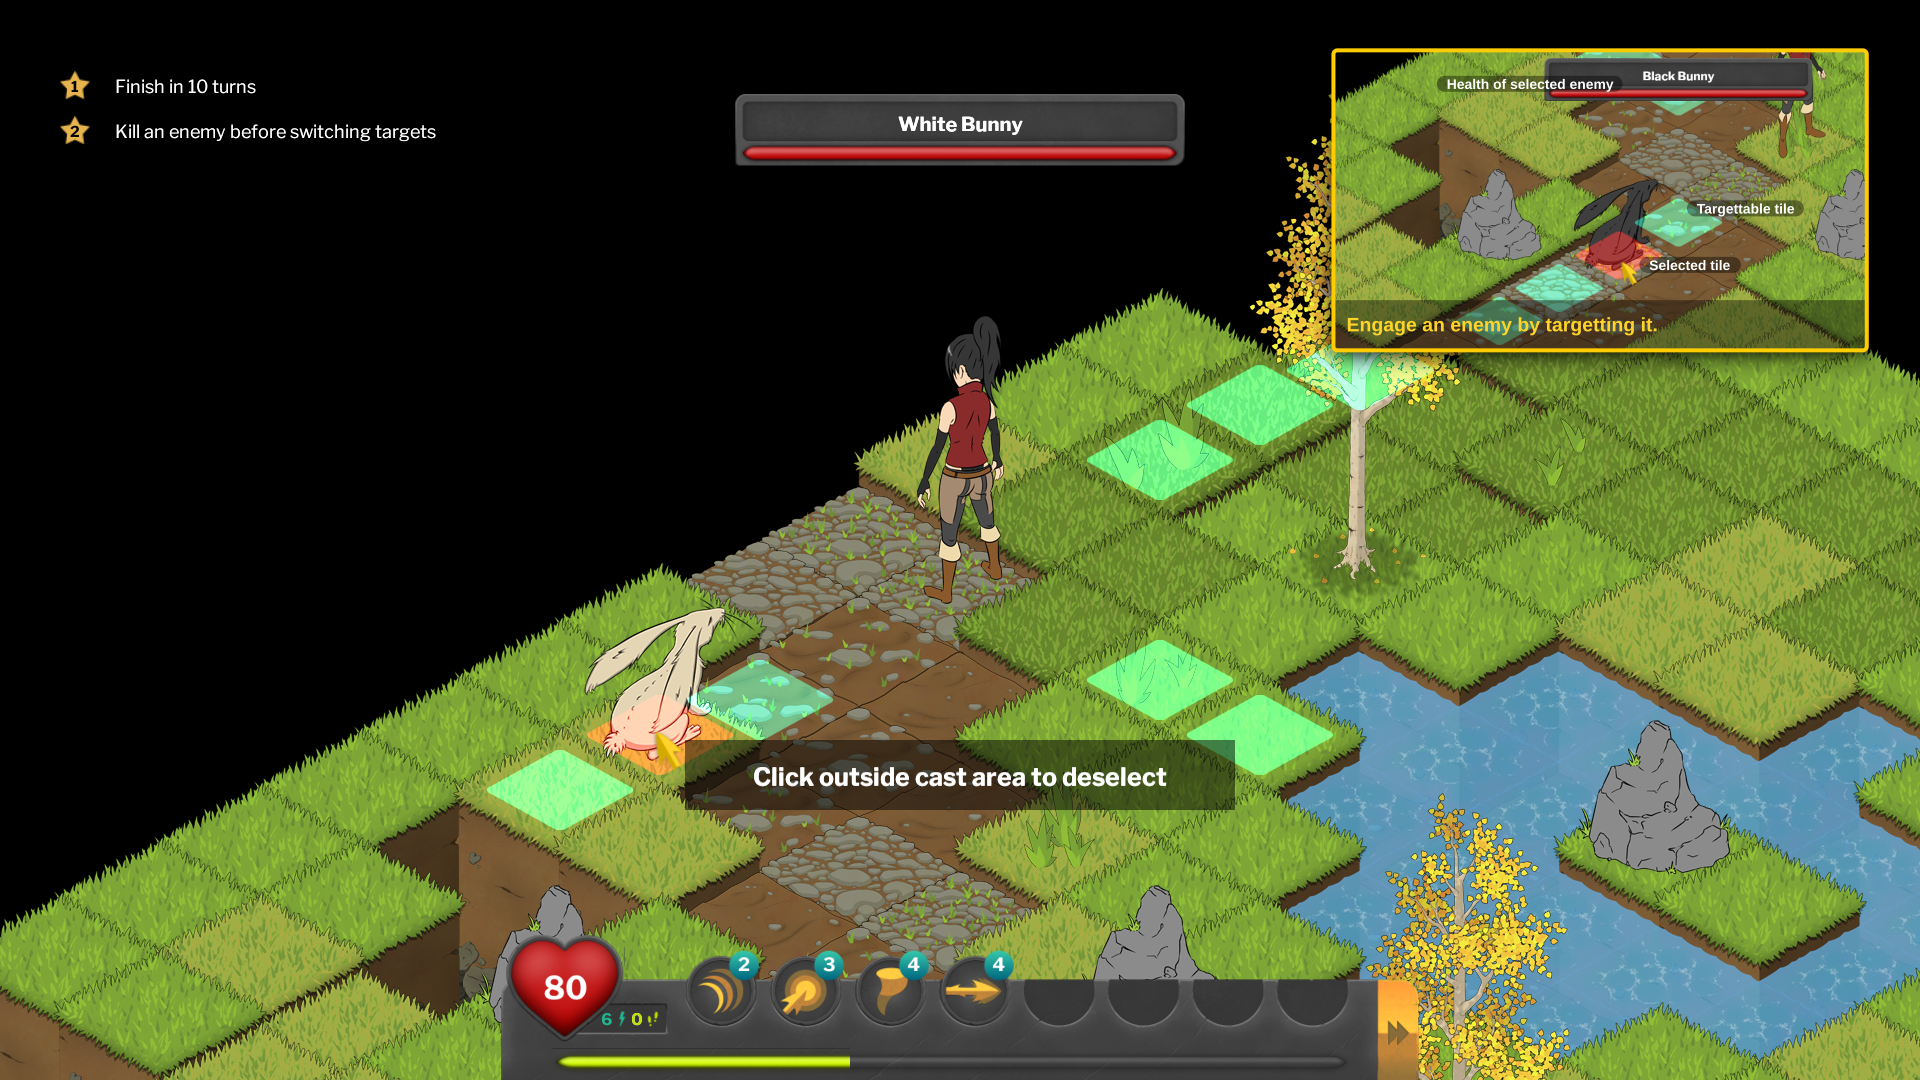
\includegraphics[scale=0.2]{tutorial}
\caption{In-game screenshot of the new player experience}
\label{fig:tutorial}
\end{figure}

\section{Steps}

\subsection{Exploration mode (first part)}
The tutorial begins immediately after starting a new game.

\begin{enumerate}
\item The first picture shows the player how to open the kanji encyclopedia GUI.
\item After opening the panel they are presented with their first kanji character and told they have to remember the furigana as it will be used in their first battle.
\item On closing the dialogue, the player receives a hint on how to move in~the~exploration mode.
\item When the player moves to another tile, they are told to talk to a nearby NPC who will offer them their first quest.
\item After accepting the quest the player is then guided to open up the~quest~GUI.
\item A brief explanation of quest types and objectives follows.
\item After closing the dialogue, the player is told to attack their first enemy, which is incidentally an objective of their first quest.
\end{enumerate}

\newpage

\subsection{Battle mode}

\begin{enumerate}
\setcounter{enumi}{7}
\item Upon entering the battle mode, the player is given instructions on~movement.
\item After moving one or more tiles, the player is told about spells and core battle mechanics (movement and action points). They are then told to~activate a spell.
\item After clicking on a spell icon, the player is instructed to choose a target.
\item Afterwards a query interface appears and the player is given an~explanation about query-specific GUI elements.
\item Upon answering the query, the player is told to end their turn.
\item After clicking on the end turn button, the player is instructed to finish the battle by defeating all enemies.
\end{enumerate}

\subsection{Exploration mode (second part)}

\begin{enumerate}
\setcounter{enumi}{13}
\item After the player emerges victorious in their first battle, they are given instructions on how to finish their quest.
\item Once they turn in the quest, they are given an explanation of~quest~rewards after which they are told to open up the inventory GUI.
\item Afterwards the differences between item types is explained and the~player is told to use their reward item, which is a~piece~of~ equipment.
\item After equipping the article of clothing, they are told about a follow-up quest, which concerns battle challenges.
\item An explanation of the challenges system follows.
\end{enumerate}

Upon completion of a single challenge, the tutorial ends.

\chapter{Testing}

\tolerance=1
\emergencystretch=\maxdimen
\hyphenpenalty=10000
\hbadness=10000

Three individuals were selected to test an unfinished prototype featuring the~first two quests. The focus of our play testing sessions was primarily on~usability and accessibility. As the graphical part of the user interface hadn't been finished at that time, we wanted to use this opportunity to analyse which elements were often overlooked in order to pass the resulting information onto~David, our graphics designer. Secondly, we were looking for both minor and game-breaking bugs.

\section{Setting}

All three individuals had previously mastered basics of Japanese, including knowledge of hiragana. Two individuals had prior experiences with an earlier build of the game, which contained some, but not all battle mechanics. One~individual did not have any prior experience with the game and for~the~rest~of~the~testing group, this was their first experience with the~exploration portion of the game.

\newpage

Testing was conducted on two different machines running the following operating systems:

\begin{itemize}
\item elementaryOS 0.4 ``Loki''
\item macOS 10.12 ``Sierra''
\end{itemize}

In addition to the three testing sessions, we have briefly tested the game on~three additional operating systems:

\begin{itemize}
\item Windows 7
\item Windows 8.1
\item Windows 10
\end{itemize}

\section{Results}

Sessions were each 15 to 20 minutes in length with testers reacting positively to the overall gameplay experience. We have divided this section into four subsections. The first two sections include technical issues encountered, the~third talks about game design issues that need to be resolved and the fourth relates to issues regarding user experience.

\subsection{Critical bugs}

The game has issues with \emph{display scaling} in Windows 10. When scaling is~enabled, the game window either does not fully display or displays partially on a secondary display. This practically limits the use on HiDPI machines running the OS. We did not encounter the issue on machines running macOS, Linux or earlier versions of Windows operating system. We have notified the~developers about this behaviour.

Another critical issue regarding the game engine used is the \emph{inability to~dynamically~set a resolution} on runtime. The game is currently hard coded to~run at a resolution of 1920 by 1080 pixels. If a user attempts to launch the~game on a system with a lower resolution, it causes the game to crash on~startup. There are two possible ways to solve this issue. 

One is to create a~launcher application which would allow the user to select an appropriate resolution prior to launching the game, an approach used heavily by~videogames built using the Unity game engine. The other is to wait for an~official roll-out of the Native Extensions system, which should allow for~writing code that utilises OS-specific APIs in order to obtain a supported resolution.

\subsection{Minor bugs}

\begin{itemize}
\item When an enemy moves, it can sometime pass the player without attacking them.
\item The camera moves abruptly, which can distract the player.
\item To interact with enemies and NPCs, the player has to click on the tile the~character is located on.
\item The player automatically initiates unwanted conversations with NPCs that are located en-route to target.
\end{itemize}

\subsection{Game design issues}

\begin{itemize}
\item The game would benefit from having AoE spells with diagonal targets. In~the current state, the player sometimes has no choice but to~end~the~turn without attacking.
\item The damage output of more expensive spells should be increased in order to motivate the player to use them more often.
\end{itemize}

\newpage

\subsection{User experience}

\begin{itemize}
\item The tutorial should limit possible movement during the first battle. It is possible for the player to reach a tile diagonal to the enemy, which leaves the player with no option but to end the turn, thus breaking the tutorial's flow.
\item Players often do not pay enough attention to NPC dialogues, which can create confusing experiences for the player if an NPC instructs them to~visit another NPC in order to continue the quest chain.
\item Two testers have made repeated mistakes while answering queries related to parsing a trailing `n' character. The parser should be modified to convert a trailing `n' character to the corresponding hiragana character (ん).
\item One tester thought the game wanted them to enter on'yomi or~kun'yomi readings of individual characters rather than readings of~kanji compounds. The interface has been redesigned to accommodate this issue by including on'yomi and kun'yomi readings on the back of~a~rotating tablet element as these readings are complementary to~the~gameplay experience.
\item One tester had issues navigating the map. The use of isometric perspective means that the player has two possible ways to interpret a~cardinal direction. This issue will be partially solved by implementing a~map interface in the future version of the game.
\end{itemize}

\chapter{Future additions}

\tolerance=1
\emergencystretch=\maxdimen
\hyphenpenalty=10000
\hbadness=10000

This chapter details some of many possible ways of improving the game.

\section{Crafting system}

Crafting system will play a large role in the game's economy. It will introduce the ability to combine resources into consumables and equipment. The~crafting update will also introduce resource nodes, which provide additional means of~\emph{generating resources}, in addition to quests and spoils of~battle. The process of gathering from a resource node will involve answering a query similar to~the~one used in battle. This provides the player with an option to~practice without significant consequences for failure.

\section{Expansions}

Expansions will typically introduce new sets of kanji characters into the~game, new gameplay areas and quests. We believe the expansions should be offered as~a~stand-alone product so that players with intermediate knowledge of~Japanese can skip the learning process for kanji they have already memorized. However, we think the expansions should introduce a~gameplay mechanic for~\emph{practising kanji} from previous expansions and the~base game. Although they can be played through in any order, the~persistence module will keep track of~progress across all expansions.

\section{Multiplayer}

One interesting functionality an expansion can bring is the addition of~a~multiplayer element. There are two possible approaches. The first is to~introduce \emph{player profiles}, which would contain achievements and statistical data such as the list of most challenging kanji for that particular player. The~second is to allow for \emph{player vs. player} combat, \emph{cooperative play} and~other complex functionality.

\section{Other versions}

As the game's design is modular, it would be very easy to create a Chinese version of the game that uses \emph{Pinyin romanization} instead of hiragana. We also have plans for a demo, which would teach the player hiragana characters, thus making the game more accessible to complete beginners in Japanese.

\begin{conclusion}

\tolerance=1
\emergencystretch=\maxdimen
\hyphenpenalty=10000
\hbadness=10000

The purpose of this thesis was to analyse existing educational products from both gaming and non-gaming backgrounds and draw from their expertise whilst creating an educational turn-based RPG of our own. We took inspiration from a number of different educational products as well as two existing videogames from the chosen genre, and specified requirements for~our game. In~subsequent chapters, we have discussed the design choices behind the~game's exploration and battle systems. We have discussed in detail various types of~quests that can be implemented in the game and the need to include variability in the quest system, as well as item types present in the game and their place within the game economy.

As part of the thesis, we have built a prototype of the game featuring one in-game area using Defold game engine and Tiled map editor. We subsequently created a tutorial system to help the player take their first steps within the game world and tested the prototype on three individuals. The testing phase helped in revealing many bugs, game design and user experience issues, which have been detailed in the corresponding section. Lastly, we shared a number of ways on how to improve the game.

Overall, I am pleased with the result, although the game still has a long way to~go in terms of both level design and game mechanics. I am working with the team behind Defold game engine in fixing the critical bugs. The research has given me valuable insight in processes involved in game design as well as software architecture in general.

\end{conclusion}

\printbibliography[title={Sources}]

\appendix

\chapter{List of abbreviations used}
% \printglossaries
\begin{description}
\item[AI] Artificial intelligence
\item[AP] Action points
\item[API] Application Programming Interface
\item[AoE] Area of effect
\item[CSV] Comma-separated values
\item[(G)UI] (Graphical) user interface
\item[HTML] Hypertext Markup Language
\item[HTTP] Hypertext Transfer Protocol
\item[HiDPI] High Dots Per Inch
\item[IDE] Integrated Development Environment
\item[(J)RPG] (Japanese) role-playing game
\item[JSON] JavaScript Object Notation
\item[NPC] Non-playable character
\item[OS] Operating system
\item[VCS] Version control system
\end{description}

\chapter{Contents of included CD}

\begin{figure}
	\dirtree{%
		.1 readme.md\DTcomment{brief overview of CD contents}.
		.1 bin\DTcomment{directory containing binaries of the game}.
		.1 cheatsheet.pdf\DTcomment{information for users with no knowledge of Japanese}.
		.1 struct\DTcomment{directory containing data structures used in the game}.
		.1 thesis\DTcomment{source of the thesis in \LaTeX{} format}.
		.1 thesis.pdf\DTcomment{thesis in PDF format}.
	}
\end{figure}

\end{document}
